\documentclass[
	% -- opções da classe memoir --
	12pt,				% tamanho da fonte
	openright,			% capítulos começam em pág ímpar (insere página vazia caso preciso)
	oneside,			% twoside para impressão em verso e anverso. Oposto a oneside
	a4paper,			% tamanho do papel. 
	% -- opções da classe dc-uel --
	dissertacao,			% tipo do trabalho (opções: tcc, tccpreliminar, dissertacao, qualificacaoms)
					% - tcc (Versão para a Banca do TCC ou Versão Final do TCC)
					% - tccpreliminar (Versão Preliminar do TCC)
					% - dissertação (Versão para a Banca da Dissertação ou Versão Final/Revisada da Dissertação)
					% - qualificacaoms (Qualificação de Mestrado)
	]{ABNT-DC-UEL}


% ---
% PACOTES
% ---

% ---
% Pacotes fundamentais 
% ---
\usepackage[T1]{fontenc}		% Selecao de codigos de fonte.
\usepackage[utf8]{inputenc}		% Codificacao do documento (conversão automática dos acentos)
\usepackage{graphicx}			% Inclusão de gráficos
\usepackage{pdfpages}			% Inclusão de (páginas de) arquivos PDF no documento
\usepackage{amssymb}			% Símbolos matemáticos (e.g. \mathbb)
% ---
		
% ---
% Pacotes adicionais, usados apenas no âmbito do Modelo Canônico do abnteX2
% ---
\usepackage{lipsum}				% para geração de dummy text
% ---

% ---
% Informações de dados para CAPA, FOLHA DE ROSTO e outros elementos
% ---
\titulo{Utilização de Small Language Models com conhecimento de domínio e Large Language Models em sistemas multiagentes para interfaces Text-to-SQL}
\tituloingles{Utilization of Small Language Models with domain knowledge and Large Language Models in multi-agent systems for Text-to-SQL interfaces.}
\palavraschave{Modelos de Linguagem. Sistemas Multiagentes. Text-to-SQL.}
\palavraschaveingles{Language Models. Multi-agent Systems. Text-to-SQL.}
\autor{Ewerthon José Kutz}
\citacaoautor{Kutz, E. J.}
\data{2026}

\diadefesa{Data TBD}
\orientador{Profa. Dra. Helen Cristina de M. Senefonte} % É membro nato e presidente da Banca Examinadora
\coorientador{Prof(a). Dr(a). Nome do(a) Coorientador(a)} % Pode ou não ser membro da Banca; se for, deve ser incluído como membro a seguir
\membrobancadois{Prof. Dr. Segundo Membro da Banca}
\instmembrobancadois{Universidade/Instituição do Segundo Membro da Banca -- Sigla instituição}
\membrobancatres{Prof. Dr. Terceiro Membro da Banca}
\instmembrobancatres{Universidade/Instituição do Terceiro Membro da Banca -- Sigla instituição}
\membrobancaquatro{Prof. Ms. Quarto Membro da Banca}
\instmembrobancaquatro{Universidade/Instituição do Quarto Membro da Banca -- Sigla instituição}

% ---
% compila o indice
% ---
\makeindex
% ---

% ----
% Início do documento
% ----
\begin{document}

% Retira espaço extra obsoleto entre as frases.
\frenchspacing

% ----------------------------------------------------------
% ELEMENTOS PRÉ-TEXTUAIS
% ----------------------------------------------------------
% \pretextual

% ---
% Capa (elemento obrigatório)
% ---
\imprimircapa
% ---

% ---
% Folha de rosto (elemento obrigatório)
% (o * indica que haverá a ficha bibliográfica)
% ---
\imprimirfolhaderosto*
% ---

% ---
% Ficha bibliografica (elemento obrigatório para versões finais de TCC e dissertação)
% ---

% Isto é um exemplo de Ficha Catalográfica, ou ``Dados internacionais de
% catalogação-na-publicação''. Você poderá utilizar o site da biblioteca para 
% gerar esta ficha através do link: http://www.uel.br/bc/ficha/. Quando estiver
% com o documento, salve-o como PDF no diretório do seu projeto e substitua todo
% o conteúdo de implementação deste arquivo pelo comando abaixo:
%
\begin{fichacatalografica}
  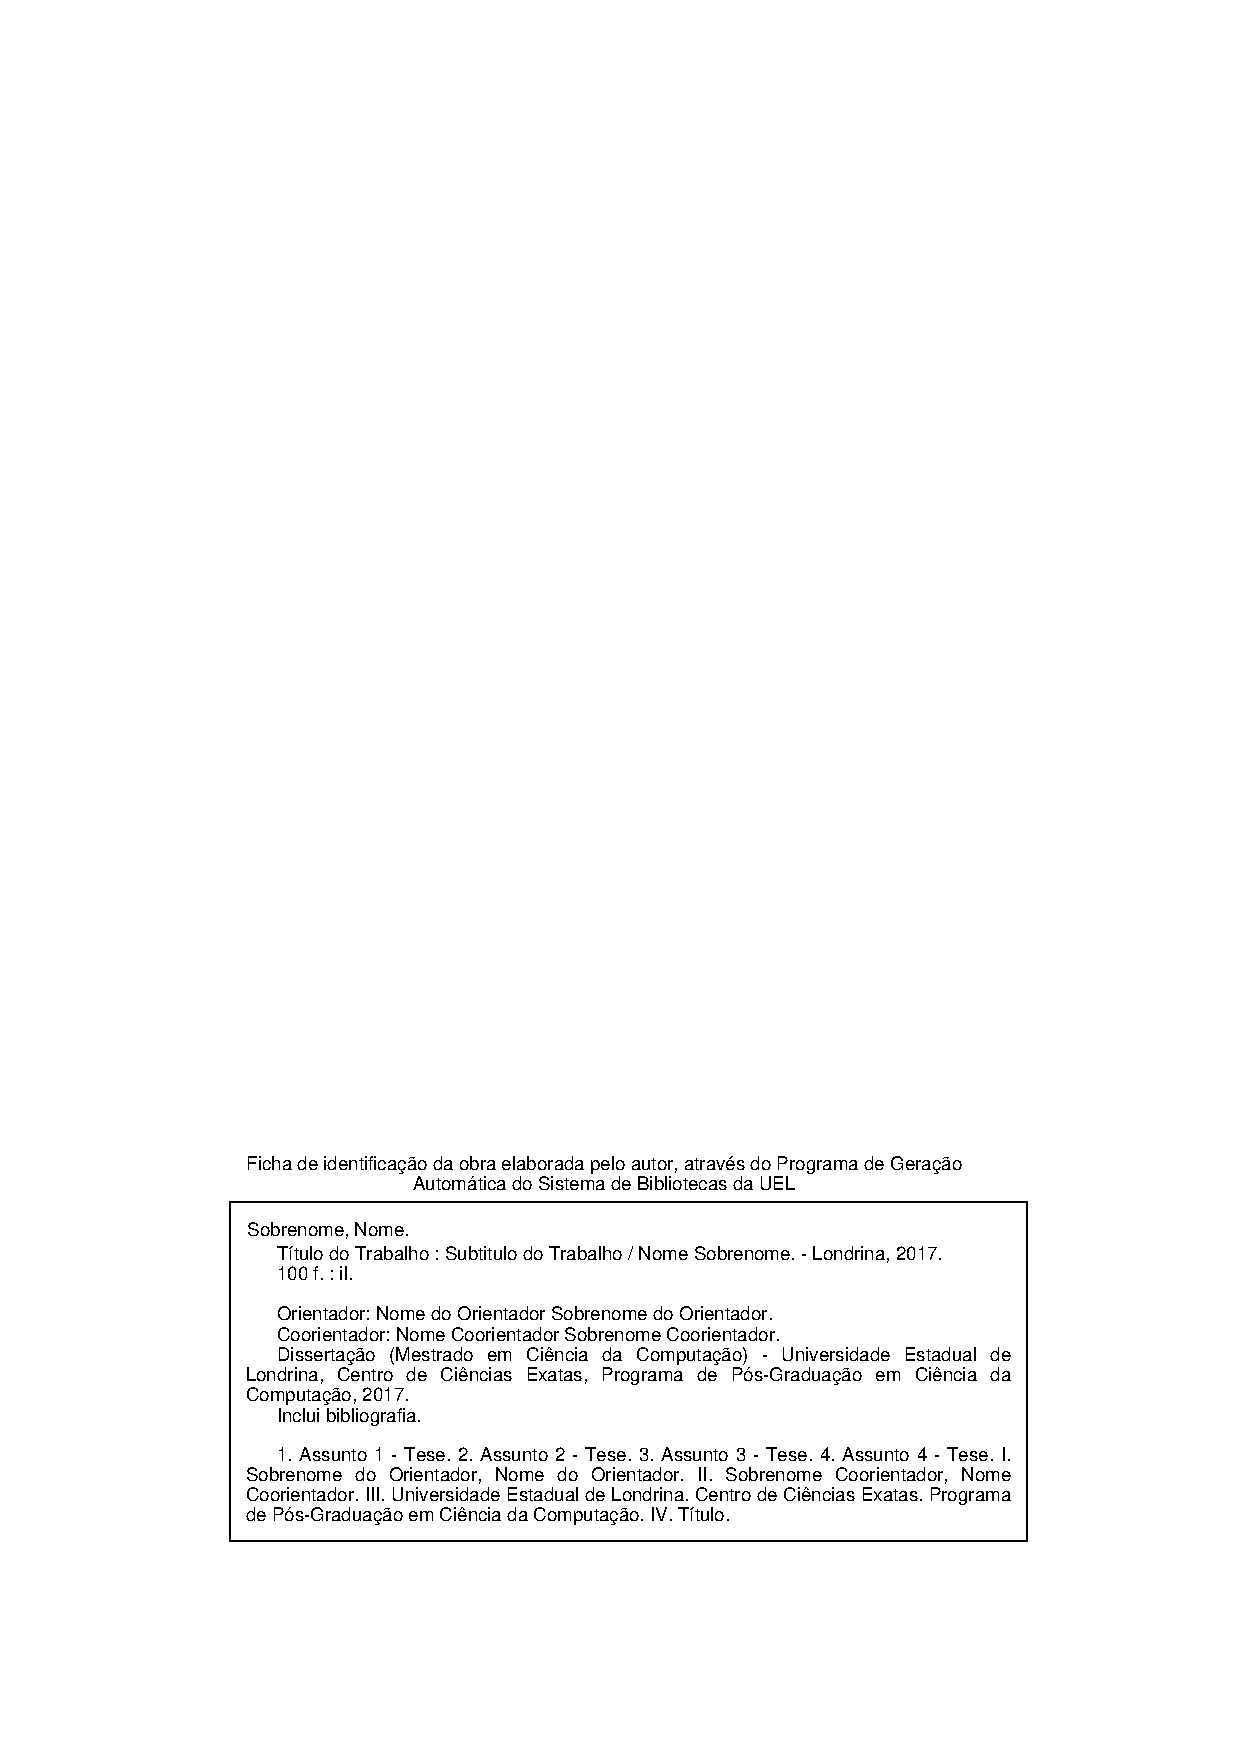
\includepdf{ficha_catalografica.pdf}
\end{fichacatalografica}


% ---

% ---
% Folha de aprovação (elemento obrigatório) ==> deve ser omitida no caso de tccpreliminar
% ---

% Isto é um exemplo de Folha de aprovação, elemento obrigatório da NBR
% 14724/2011 (seção 4.2.1.3). Você pode utilizar este modelo até a aprovação
% do trabalho. Após isso, substitua todo o conteúdo deste arquivo por uma
% imagem da página assinada pela banca com o comando abaixo:
%
% \includepdf{folhadeaprovacao_final.pdf}
\imprimirfolhadeaprovacao
% ---

% ---
% Dedicatória (elemento opcional)
% ---
\begin{dedicatoria}
  \vspace*{\fill}
  \hspace{.4\textwidth}
  \begin{minipage}{.5\textwidth}
    \begin{flushright}
      \textit{Este trabalho é dedicado às crianças adultas que, quando pequenas, sonharam em se tornar cientistas.}
    \end{flushright}
  \end{minipage}
\end{dedicatoria}
% ---

% ---
% Agradecimentos (elemento opcional, mas fortemente recomendado)
% ---
\begin{agradecimentos}
  Os agradecimentos principais são direcionados à Gerald Weber, Miguel Frasson,
  Leslie H. Watter, Bruno Parente Lima, Flávio de Vasconcellos Corrêa, Otavio Real
  Salvador, Renato Machnievscz\footnote{Os nomes dos integrantes do primeiro
    projeto abn\TeX\ foram extraídos de
    \url{http://codigolivre.org.br/projects/abntex/}} e todos aqueles que
  contribuíram para que a produção de trabalhos acadêmicos conforme
  as normas ABNT com \LaTeX\ fosse possível.

  Agradecimentos especiais são direcionados ao Centro de Pesquisa em Arquitetura
  da Informação\footnote{\url{http://www.cpai.unb.br/}} da Universidade de
  Brasília (CPAI), ao grupo de usuários
  \emph{latex-br}\footnote{\url{http://groups.google.com/group/latex-br}} e aos
  novos voluntários do grupo
  \emph{\abnTeX}\footnote{\url{http://groups.google.com/group/abntex2} e
    \url{http://abntex2.googlecode.com/}}~que contribuíram e que ainda
  contribuirão para a evolução do \abnTeX.

\end{agradecimentos}
% ---

% ---
% Epígrafe (elemento opcional)
% ---
\begin{epigrafe}
  \vspace*{\fill}
  \hspace{.4\textwidth}
  \begin{minipage}{.5\textwidth}
    \begin{flushright}
      \textit{
        ``Não vos amoldeis às estruturas deste mundo,
        mas transformai-vos pela renovação da mente,
        a fim de distinguir qual é a vontade de Deus:
        o que é bom, o que Lhe é agradável, o que é perfeito.\\
        (Bíblia Sagrada, Romanos 12, 2))}
    \end{flushright}
  \end{minipage}
\end{epigrafe}
% ---

% ---
% RESUMOS
% ---

% ---
% Resumo em Português (elemento obrigatório)
% ---
\begin{resumo}
  Os recentes avanços em inteligência artificial têm impulsionado o uso de modelos de linguagem generativos de formas complexas e em aplicações cada vez mais avançadas, incluindo o uso de Large Language Models (LLMs) como agentes em sistemas inteligentes. Este trabalho propõe utilizar Small Language Models (SLMs) com conhecimento de domínio em comparação a LLMs em sistemas multiagentes colaborativos em interfaces Text-To-SQL. Para isso, esses modelos serão ajustados com métodos como qLoRA e few-shot prompting e avaliados como agentes em métricas de acurácia, corretude e custo-benefício por meio de datasets de interface de linguagem natural para SQL. Espera-se validar o uso de SLMs como uma solução eficaz frente a modelos maiores e mais custosos, além de desenvolver um framework de agentes colaborativos que pode ser reutilizado em outras aplicações.
\end{resumo}
% ---

% ---
% Resumo em Inglês (elemento obrigatório)
% ---
% O ambiente Abstract (com A maiúsculo) é definido no estilo dc-uel
\begin{Abstract}
  Recent advances in artificial intelligence have driven the use of generative language models in increasingly complex and advanced applications, including the deployment of Large Language Models (LLMs) as agents in intelligent systems. This work proposes the use of Small Language Models (SLMs) with domain knowledge, in comparison to LLMs, within collaborative multi-agent systems in Text-to-SQL interfaces. To achieve this, these models will be fine-tuned using methods such as qLoRA and few-shot prompting and evaluated as agents based on accuracy, correctness, and cost-effectiveness metrics using datasets designed for natural language to SQL interfaces. The expected outcome is to validate the use of SLMs as an effective solution compared to larger, more costly models, as well as to develop a collaborative agents framework that can be reused in other applications.
\end{Abstract}
% ---

% ---
% Lista de ilustrações (elemento opcional, mas fortemente recomendado)
% ---
\pdfbookmark[0]{\listfigurename}{lof}
\listoffigures*
\cleardoublepage
% ---

% ---
% Lista de tabelas (elemento opcional, mas fortemente recomendado)
% ---
\pdfbookmark[0]{\listtablename}{lot}
\listoftables*
\cleardoublepage
% ---

% ---
% Lista de abreviaturas e siglas (elemento opcional)
% ---
\begin{siglas}
  \item[ABNT] Associação Brasileira de Normas Técnicas
  \item[BNDES] Banco Nacional de Desenvolvimento Econômico e Social
  \item[IBGE] Instituto Nacional de Geografia e Estatística
  \item[IBICT] Instituto Brasileiro de Informação em Ciência e Tecnologia
  \item[NBR] Norma Brasileira
\end{siglas}
% ---

% ---
% Lista de símbolos (elemento opcional)
% ---
% \begin{simbolos}
%   \item[$ \Gamma $] Letra grega Gama
%   \item[$ \Lambda $] Lambda
%   \item[$ \zeta $] Letra grega minúscula zeta
%   \item[$ \in $] Pertence
% \end{simbolos}
% ---

% ---
% Sumario (elemento obrigatório)
% ---
\pdfbookmark[0]{\contentsname}{toc}
\tableofcontents*
\cleardoublepage
% ---

% ----------------------------------------------------------
% ELEMENTOS TEXTUAIS
% ----------------------------------------------------------
\textual
\pagestyle{dc-uel-header} % Configura cabeçalho para apresentar apenas números de página

% ----------------------------------------------------------
% Introdução
% ----------------------------------------------------------
\chapter{Introdução}

Este documento e seu código-fonte são uma pequena adaptação do exemplo de uso fornecido pela equipe desenvolvedora da classe \textsf{abntex2}, atendendo a particularidades inseridas na classe \textsf{ABNT-DC-UEL.cls} que define o modelo para Trabalhos de Conclusão de Curso e Dissertações de Mestrado dos cursos do Departamento de Computação da Universidade Estadual de Londrina. Observe-se que o documento está preparado para impressão em frente e verso (opções twoside e openright) e que para gerar o índice remissivo deve-se utilizar o comando \textsf{makeindex}. Sugestões de melhorias ou problemas encontrados, favor notificar (Prof. Daniel S. Kaster -- \href{mailto:dskaster@uel.br}{dskaster@uel.br}).

Este documento e seu código-fonte são exemplos de referência de uso da classe \textsf{abntex2} e do pacote \textsf{abntex2cite}. O documento exemplifica a elaboração de trabalho acadêmico (tese, dissertação e outros do gênero) produzido conforme a ABNT NBR 14724:2011 \emph{Informação e documentação - Trabalhos acadêmicos - Apresentação}.

A expressão ``Modelo Canônico'' é utilizada para indicar que \abnTeX\ não é modelo específico de nenhuma universidade ou instituição, mas que implementa tão somente os requisitos das normas da ABNT. Uma lista completa das normas observadas pelo \abnTeX\ é apresentada em \citeonline{abntex2classe}.

Sinta-se convidado a participar do projeto \abnTeX! Acesse o site do projeto em \url{http://abntex2.googlecode.com/}. Também fique livre para conhecer, estudar, alterar e redistribuir o trabalho do \abnTeX, desde que os arquivos modificados tenham seus nomes alterados e que os créditos sejam dados aos autores originais, nos termos da ``The \LaTeX\ Project Public License''\footnote{\url{http://www.latex-project.org/lppl.txt}}.

Encorajamos que sejam realizadas customizações específicas deste exemplo para universidades e outras instituições --- como capas, folha de aprovação, etc. Porém, recomendamos que ao invés de se alterar diretamente os arquivos do \abnTeX, distribua-se arquivos com as respectivas customizações. Isso permite que futuras versões do \abnTeX~não se tornem automaticamente incompatíveis com as customizações promovidas. Consulte \citeonline{abntex2-wiki-como-customizar} par mais informações.

Este documento deve ser utilizado como complemento dos manuais do \abnTeX\
\cite{abntex2classe,abntex2cite,abntex2cite-alf} e da classe \textsf{memoir}
\cite{memoir}.

Esperamos, sinceramente, que o \abnTeX\ aprimore a qualidade do trabalho que você produzirá, de modo que o principal esforço seja concentrado no principal: na contribuição científica.

Equipe \abnTeX

Lauro César Araujo

% ----------------------------------------------------------
% Capitulo com exemplos de comandos inseridos de arquivo externo 
% ----------------------------------------------------------

\include{commands}

\chapter{Fundamentação Teórica}

\section{Modelos de Linguagem}

Um modelo de linguagem computacional consiste em um sistema probabilístico capaz de prever a próxima unidade de texto em uma sequência, condicionada às anteriores \cite{caseli2024}. Embora frequentemente referidas como "palavras", as unidades fundamentais processadas pelos modelos modernos denominam-se \textit{tokens}. Estes podem representar palavras inteiras, subpalavras ou caracteres, tornando a \textit{tokenização} a etapa primária de engenharia de características \cite{raff2025,caseli2024}. Para o processamento, tais \textit{tokens} são convertidos em vetores numéricos multidimensionais. Dada a complexidade linguística, uma representação simples desse espaço resulta em vetores de altíssima dimensionalidade e esparsidade e torna seu processamento uma tarefa extremamente complexa, fenômeno conhecido como a "maldição da dimensionalidade" \cite{raff2025}.

Historicamente, abordagens iniciais como o \textit{Bag-of-Words} (BoW) tratavam o texto apenas como uma contagem de frequência, ignorando a ordem sequencial e a estrutura sintática \cite{amaratunga2023}. A superação dessa limitação ocorreu com o desenvolvimento de representações distribuídas, fundamentadas na hipótese distribucional de linguistas como Harris e Firth (década de 1950), que postula que palavras em contextos similares compartilham significados semelhantes \cite{jurafsky2025}. Contudo, essas representações ganharam viabilidade prática apenas recentemente com técnicas eficientes como o Word2Vec, que consolidaram o uso de \textit{embeddings} \cite{caseli2024, goodfellow2016}.

Os Modelos de Linguagem Neurais (NLMs) operam sobre esse espaço vetorial denso, onde a distância euclidiana entre os vetores reflete a similaridade semântica entre os termos. Diferentemente dos modelos de contagem, os NLMs generalizam o aprendizado: ao identificar que dois \textit{tokens} compartilham contextos vetoriais próximos, o modelo transfere o conhecimento de um para o outro \cite{goodfellow2016}. Os \textit{embeddings}, portanto, solucionam o problema da dimensionalidade ao projetar o vocabulário em um espaço contínuo de baixa dimensão, capturando relações semânticas complexas \cite{amaratunga2023}, conforme ilustrado na Figura \ref{fig:espaco_semantico}.

\begin{figure}[htb]
  \centering
  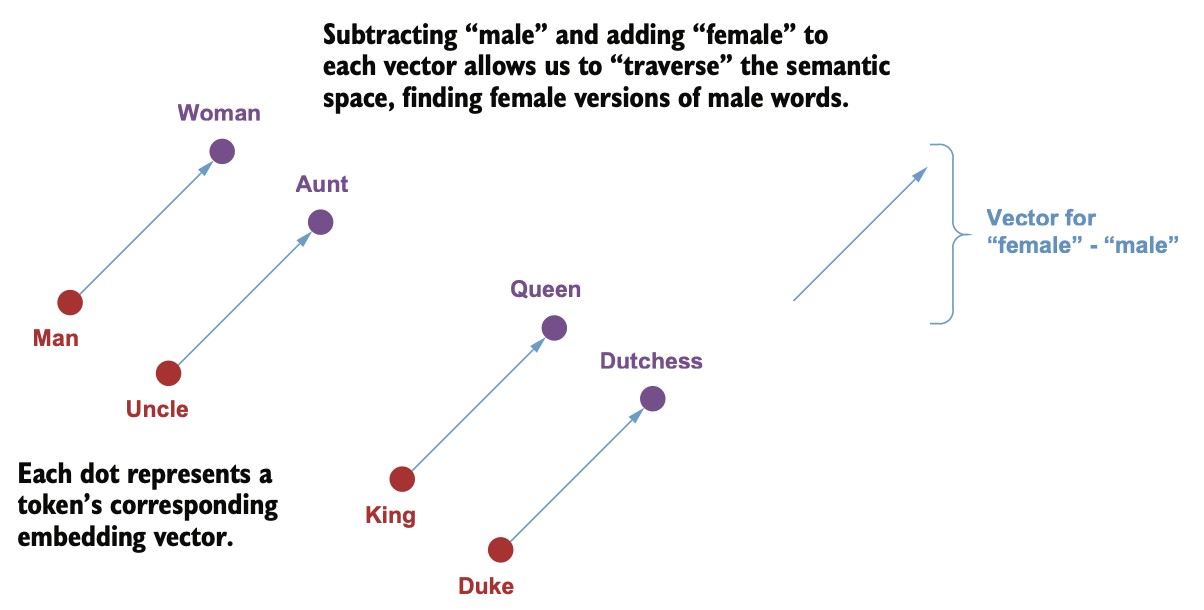
\includegraphics[scale=0.6]{images/raff2025_espaco_semantico.png}
  \caption{Espaço semântico e vetorial. Fonte: \cite{raff2025}.}
  \label{fig:espaco_semantico}
\end{figure}

A natureza algébrica dos \textit{embeddings} permite operações vetoriais que refletem analogias linguísticas — como a clássica operação "rei - homem + mulher = rainha" — e a identificação de sinonímia que modelos baseados em contagem tratariam como entidades disjuntas \cite{caseli2024,amaratunga2023}.

Em 2017, a introdução da arquitetura \textit{Transformers} estabeleceu um novo paradigma no processamento de linguagem natural \cite{amaratunga2023}. Ao contrário das Redes Neurais Recorrentes (RNNs) e LSTMs, que processam dados sequencialmente e degradam em dependências de longa distância, os \textit{Transformers} utilizam mecanismos de atenção para modelar dependências globais entre a entrada e a saída de forma paralela \cite{amaratunga2023}.

Embora a arquitetura original do \textit{Transformer} \cite{vaswani2017} integrasse blocos de codificação e decodificação, a evolução da área conduziu à especialização dessas estruturas em três categorias arquiteturais \cite{raff2025}:
\begin{itemize}
  \item \textbf{Modelos \textit{Encoder-only}} (e.g., BERT): otimizados para tarefas de compreensão e classificação;
  \item \textbf{Modelos \textit{Decoder-only}} (e.g., família GPT): focados na geração autorregressiva de texto;
  \item \textbf{Modelos \textit{Encoder-Decoder}} (e.g., T5): mantêm a estrutura híbrida para tradução e sumarização.
\end{itemize}

O fluxo de processamento nos \textit{Transformers} inicia-se na conversão dos \textit{tokens} em representações vetoriais contínuas. Uma característica intrínseca dessa arquitetura é o processamento paralelo, que confere eficiência computacional, mas remove a informação implícita de ordem sequencial \cite{caseli2024}. Para reintroduzir a noção de sequência, utilizam-se vetores de codificação posicional (\textit{positional encodings}). Estes vetores, baseados em funções senoidais ou parâmetros aprendidos, são somados aos \textit{embeddings} de entrada, permitindo que o modelo distingua a posição relativa dos termos (e.g., diferenciando sujeito de objeto) \cite{jurafsky2025}.

O mecanismo de atenção (\textit{attention mechanism}) constitui o núcleo da capacidade do \textit{Transformer} em contextualizar relações distantes. Para cada \textit{token}, o modelo aprende três projeções lineares: \textit{Query} (Q), \textit{Key} (K) e \textit{Value} (V) \cite{amaratunga2023}. Estabelece-se uma analogia desse processo com um sistema de recuperação em um "dicionário difuso" (Figura \ref{fig:dicionario_difuso}) \cite{raff2025}. Diferente de uma busca exata, a \textit{Query} de um \textit{token} é comparada probabilisticamente com as \textit{Keys} de todo o contexto para ponderar a recuperação dos valores.

\begin{figure}[htb]
  \centering
  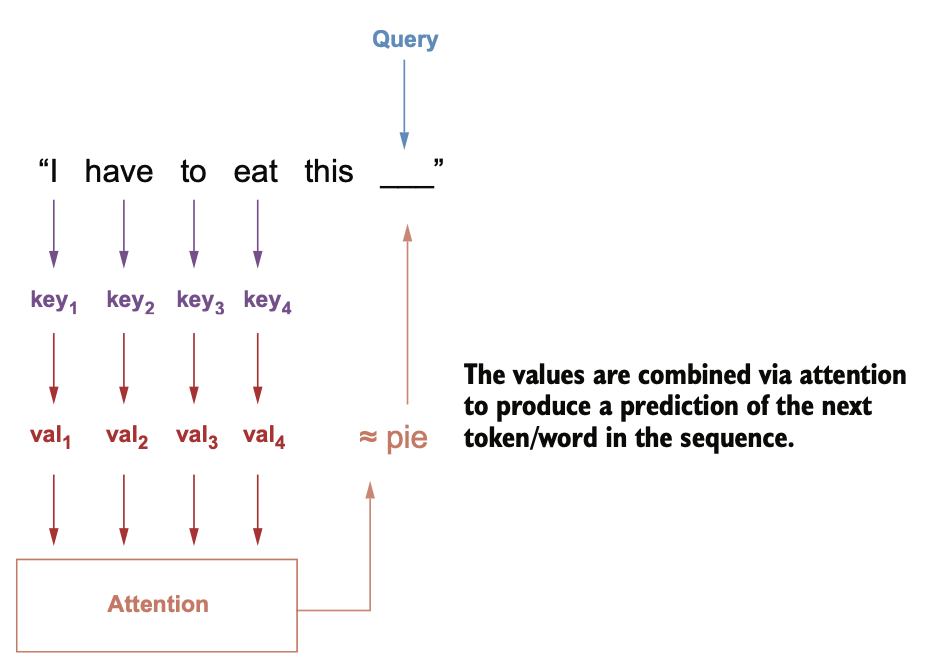
\includegraphics[scale=0.6]{images/raff2025_dicionario_difuso.png}
  \caption{Analogia do mecanismo de atenção com um dicionário difuso. Fonte: \cite{raff2025}.}
  \label{fig:dicionario_difuso}
\end{figure}

Matematicamente, essa comparação ocorre via produto escalar entre Q e K. Para garantir estabilidade numérica de gradientes, os resultados são divididos pela raiz quadrada da dimensão dos vetores ($\sqrt{d_k}$), técnica denominada \textit{Scaled Dot-Product Attention} \cite{vaswani2017}. Aplica-se então uma função \textit{softmax} para normalizar os escores em uma distribuição de probabilidade. Esses pesos resultantes ponderam a soma dos vetores \textit{Value} (V), gerando uma representação final que captura o contexto semântico completo (Figura \ref{fig:scaled_dot_product}) \cite{vaswani2017}.

\begin{figure}[htb]
  \centering
  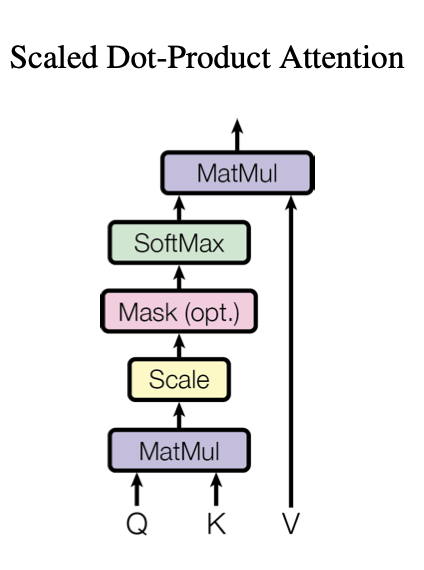
\includegraphics[scale=0.6]{images/vaswani2017_scaled_dot_product.png}
  \caption{Scaled Dot-Product Attention. Fonte: \cite{vaswani2017}.}
  \label{fig:scaled_dot_product}
\end{figure}

Para capturar simultaneamente diferentes nuances linguísticas (sintaxe, semântica, correferências), adota-se o \textit{Multi-Head Attention}. Múltiplos mecanismos ("cabeças") operam em paralelo em subespaços representacionais distintos. A concatenação e projeção linear dessas saídas proporcionam uma compreensão robusta, onde cada cabeça foca em aspectos complementares da sentença (Figura \ref{fig:multi_head_attention}) \cite{amaratunga2023, jurafsky2025}.

\begin{figure}[htb]
  \centering
  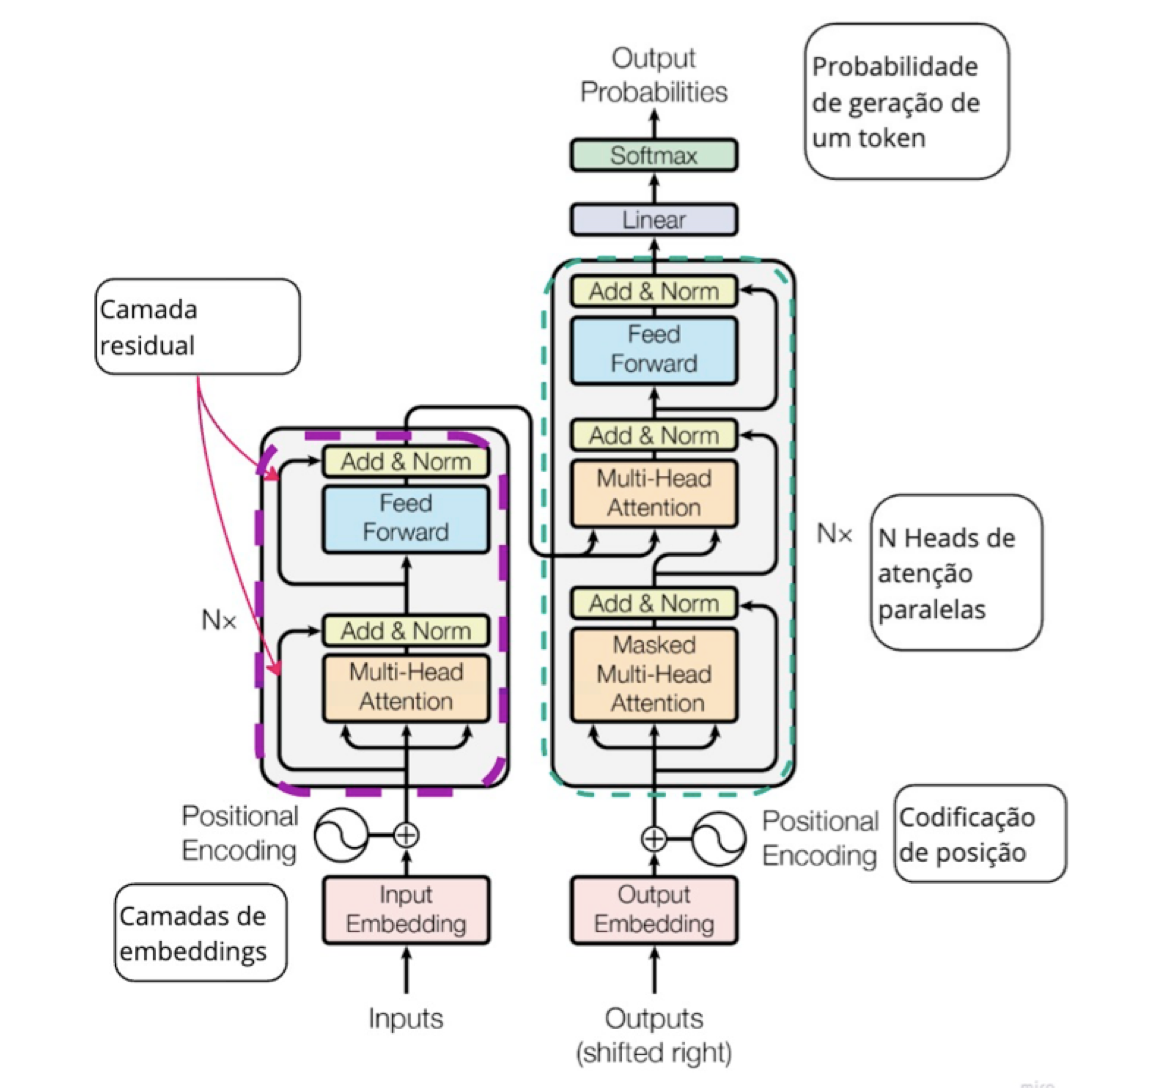
\includegraphics[scale=0.5]{images/caseli2024_atencao_multi_headed.png}
  \caption{Multi-Head Attention. Fonte: \cite{caseli2024}.}
  \label{fig:multi_head_attention}
\end{figure}

Nos modelos generativos (\textit{decoder-only}), o processo é autorregressivo. A saída das camadas do \textit{Transformer} atravessa uma etapa de \textit{unembedding} seguida de uma função \textit{softmax}, convertendo os vetores latentes em uma distribuição de probabilidade sobre o vocabulário \cite{raff2025,jurafsky2025}. A seleção final do \textit{token} depende de estratégias de amostragem (\textit{sampling}). Parâmetros como a temperatura introduzem estocasticidade, permitindo criatividade ou alucinação. A natureza não-determinística é ilustrada com o exemplo de um modelo completando a frase "I love to eat" com "chalk" (giz); caso a amostragem selecione essa opção de baixa probabilidade, o modelo tentará justificar a escolha no contexto subsequente (e.g., citando uma condição médica), demonstrando a coerência interna independente da veracidade factual \cite{raff2025}.

\section{Large Language Models e Small Language Models}

Os modelos de linguagem baseados em \textit{Transformers} representam uma nova era no Processamento de Linguagem Natural (PLN) \cite{caseli2024}. O primeiro sistema a ganhar notoriedade global, devido ao desempenho inédito em tarefas generalistas — quebrando recordes em 11 delas —, foi o BERT \cite{devlin2019}. Posteriormente, o ChatGPT 3.5 elevou essas arquiteturas ao protagonismo da Inteligência Artificial, consolidando a capacidade de diálogo por meio do ajuste fino supervisionado e do \textit{Reinforcement Learning from Human Feedback} (RLHF) \cite{ouyang2022}. Embora sem definição formal rígida, o sucesso desse sistema popularizou o conceito de \textit{Large Language Models} (LLMs), associando sua competência à escala massiva de centenas de bilhões de parâmetros.

Essa associação fundamenta-se em estudos preliminares que indicavam que o desempenho dos modelos de linguagem melhora continuamente conforme o aumento do tamanho da rede, do volume de dados e do poder computacional, obedecendo a leis de escala previsíveis \cite{kaplan2020}. Tais descobertas forneceram a justificativa científica para a corrida por modelos com centenas de bilhões de parâmetros, estabelecendo o dogma de que “maior é melhor” que dominou o desenvolvimento de LLMs nos anos subsequentes.

Adicionalmente, observa-se nesses sistemas o fenômeno das "habilidades emergentes". Trata-se de capacidades que não podem ser previstas pela extrapolação linear do desempenho de modelos menores (como o BERT): a performance permanece próxima ao aleatório até que um limiar crítico de escala seja atingido, momento em que ocorre um salto qualitativo substancial \cite{wei2022emergent}. Documentam-se múltiplos exemplos dessas emergências, incluindo raciocínio aritmético, compreensão multitarefa (MMLU) e seguimento de instruções complexas, que se manifestam tipicamente em faixas entre 10 bilhões e 500 bilhões de parâmetros, variando conforme a arquitetura \cite{wei2022emergent,zhao2025}.

Contudo, a premissa de que o aumento de escala é o único vetor de qualidade foi contestada. Evidências apontaram que muitos LLMs apresentavam sinais de "subtreinamento" como consequência do foco excessivo no tamanho do modelo em detrimento do volume e qualidade de dados. Argumenta-se que, para um treinamento computacionalmente ótimo, o tamanho do modelo e o número de \textit{tokens} de treinamento devem ser escalados proporcionalmente \cite{hoffmann2022}. A descoberta de que modelos menores, quando treinados com maior volume de dados, podem superar arquiteturas significativamente maiores desafiou as leis de escala tradicionais. O modelo Chinchilla (70B), por exemplo, superou uniformemente modelos como Gopher (280B) e GPT-3 (175B) em diversas tarefas de avaliação, utilizando quatro vezes mais dados de treino \cite{hoffmann2022}. Esses resultados estabeleceram as bases para o desenvolvimento de \textit{Small Language Models} (SLMs) especializados, sugerindo que a eficiência do treinamento e a qualidade dos dados podem compensar a redução de parâmetros.

Pesquisas subsequentes corroboraram que a "inteligência" do modelo não é apenas subproduto do volume de parâmetros. A família Llama, com arquiteturas de até 13 bilhões de parâmetros focadas em eficiência de inferência e exposição a dados de alta qualidade, superou o GPT-3 (175B) na maioria dos \textit{benchmarks}, apesar de ser treze vezes menor em número de parâmetros \cite{touvron2023}.

Paralelamente, a fundamentação da família Phi demonstrou que a "qualidade didática" dos dados permite que SLMs — definidos como modelos com menos de 10 bilhões de parâmetros — superem LLMs em raciocínio lógico e codificação \cite{gunasekar2023}. O modelo phi-1 (1,3B), por exemplo, obteve desempenho superior ao StarCoder (15,5B) no \textit{benchmark} HumanEval. Para atingir tais resultados, o ajuste fino (\textit{fine-tuning}) mostra-se crucial para desbloquear capacidades e equiparar o desempenho aos modelos massivos, tendência também observada na família Flan-T5, cuja variante de 3 bilhões de parâmetros superou o GPT-3 no \textit{benchmark} MMLU em 9\% \cite{chung2024}.

Embora os LLMs representem o estado da arte em performance bruta, os SLMs consolidam-se como alternativas promissoras devido à menor latência e à viabilidade de execução local. Essa descentralização mitiga riscos de privacidade inerentes ao processamento em nuvem, fator crítico dado que os LLMs mais potentes são proprietários e fechados \cite{wang2025llmsurvey}. Quando ajustados e aplicados a domínios específicos - como o de saúde -, SLMs com menos de 1,6 bilhão de parâmetros alcançaram 75,4\% de precisão no PubMedQA, superando os 74,4\% do GPT-4 em cenários \textit{few-shot} \cite{wang2025llmsurvey}.

Além da eficácia, os SLMs endereçam o dilema energético. Modelos menores podem atingir desempenho competitivo gerando emissões de CO$_2$ entre 660 e 13.000 vezes inferiores às de um LLM massivo \cite{garg2025}. Apesar de ainda apresentarem limitações em raciocínio complexo e generalista, a tendência atual aponta para sistemas híbridos que mesclam ambos os tipos de modelos para otimizar a relação custo-benefício \cite{zhao2025}.

A transição para modelos compactos é particularmente estratégica para sistemas de agentes de IA. A predominância atual de LLMs em agentes mostra-se muitas vezes excessiva e desalinhada com demandas de escopo restrito. Os SLMs fornecem uma alternativa viável para o futuro dessa área, baseando-se em três pilares: capacidade técnica suficiente para sub-tarefas, adequação operacional e eficiência econômica \cite{wang2025llmsurvey, belcak2025}:

\begin{itemize}
  \item \textbf{Capacidade Técnica:} SLMs modernos demonstram aptidão para tarefas críticas de agentes, como uso de ferramentas (\textit{tool calling}) e seguimento de instruções. O modelo Hymba-1.5B, por exemplo, supera modelos de 13B em precisão de instrução, enquanto a série Phi-2 (2,7B) atinge métricas de geração de código equivalentes a modelos de 30B, com velocidade 15 vezes superior \cite{belcak2025}.
  \item \textbf{Eficiência e Economia:} A inferência de um SLM de 7B é de 10 a 30 vezes mais econômica em latência e energia do que a de um LLM de 175B. Tal eficiência é vital, considerando que a inferência pode representar até 90\% do consumo energético do ciclo de vida do modelo \cite{belcak2025}.
  \item \textbf{Agilidade e Especialização:} O ajuste fino de SLMs pode ser concluído em poucas horas, permitindo a rápida integração ou correção de comportamentos, em contraste com as semanas exigidas por modelos massivos. Isso favorece arquiteturas modulares onde SLMs atuam como especialistas interagindo com LLMs centrais \cite{belcak2025}.
\end{itemize}

Apesar dos avanços, modelos baseados em \textit{Transformers} — independentemente da escala — enfrentam desafios estruturais. O custo computacional do mecanismo de atenção cresce quadraticamente com o comprimento da sequência, dificultando o processamento de contextos longos \cite{jurafsky2025}. Para SLMs, essa restrição na "janela de contexto" pode inviabilizar a execução de tarefas complexas que exigem grande recuperação de informação \cite{wang2025llmsurvey}.

Adicionalmente, o treinamento de modelos massivos demanda recursos exorbitantes. Estima-se que o treinamento do GPT-3 (175B) tenha emitido 550 toneladas métricas de CO$_2$, e com as leis de escala ainda vigentes, a demanda por recursos tende a crescer, exacerbando o impacto ambiental \cite{garg2025, zhao2025}. Questões de confiabilidade também permanecem críticas: as alucinações — geração de informações plausíveis, porém incorretas — persistem tanto em LLMs quanto em SLMs. Esse fenômeno, decorrente da natureza probabilística de previsão de \textit{tokens} e de dados ruidosos, revela uma lacuna na capacidade de monitoramento interno e verificação factual dessas ferramentas \cite{zhao2025, wang2025llmsurvey}. Por fim, a interpretabilidade permanece um desafio aberto, visto que a complexidade das redes neurais profundas dificulta a compreensão mecanística de como o modelo deriva suas respostas, mantendo o estigma de "caixas pretas" \cite{jurafsky2025}.

\section{Ajuste Fino (\textit{Fine-tuning})}

O ajuste fino constitui o método essencial para alinhar modelos de linguagem pré-treinados à intenção humana, transformando sua capacidade bruta de previsão de texto na habilidade de seguir instruções de forma útil e segura \cite{ouyang2022}. A metodologia estrutura-se em três etapas distintas: primeiramente, o \textit{Supervised Fine-Tuning} (SFT), onde o modelo é ajustado com um conjunto de dados de demonstrações humanas do comportamento desejado; em seguida, o treinamento de um Modelo de Recompensa (\textit{Reward Model}), criado a partir de comparações onde humanos classificam diferentes saídas; e, por fim, a otimização via \textit{Reinforcement Learning} utilizando o algoritmo PPO, que refina a política para maximizar a pontuação de recompensa \cite{ouyang2022}. Esse processo atua como a ponte que corrige o desalinhamento entre o objetivo de pré-treinamento e a necessidade de agir conforme as instruções do usuário, viabilizando as aplicações atuais de LLMs \cite{wei2022finetune}.

\begin{figure}[htb]
  \centering
  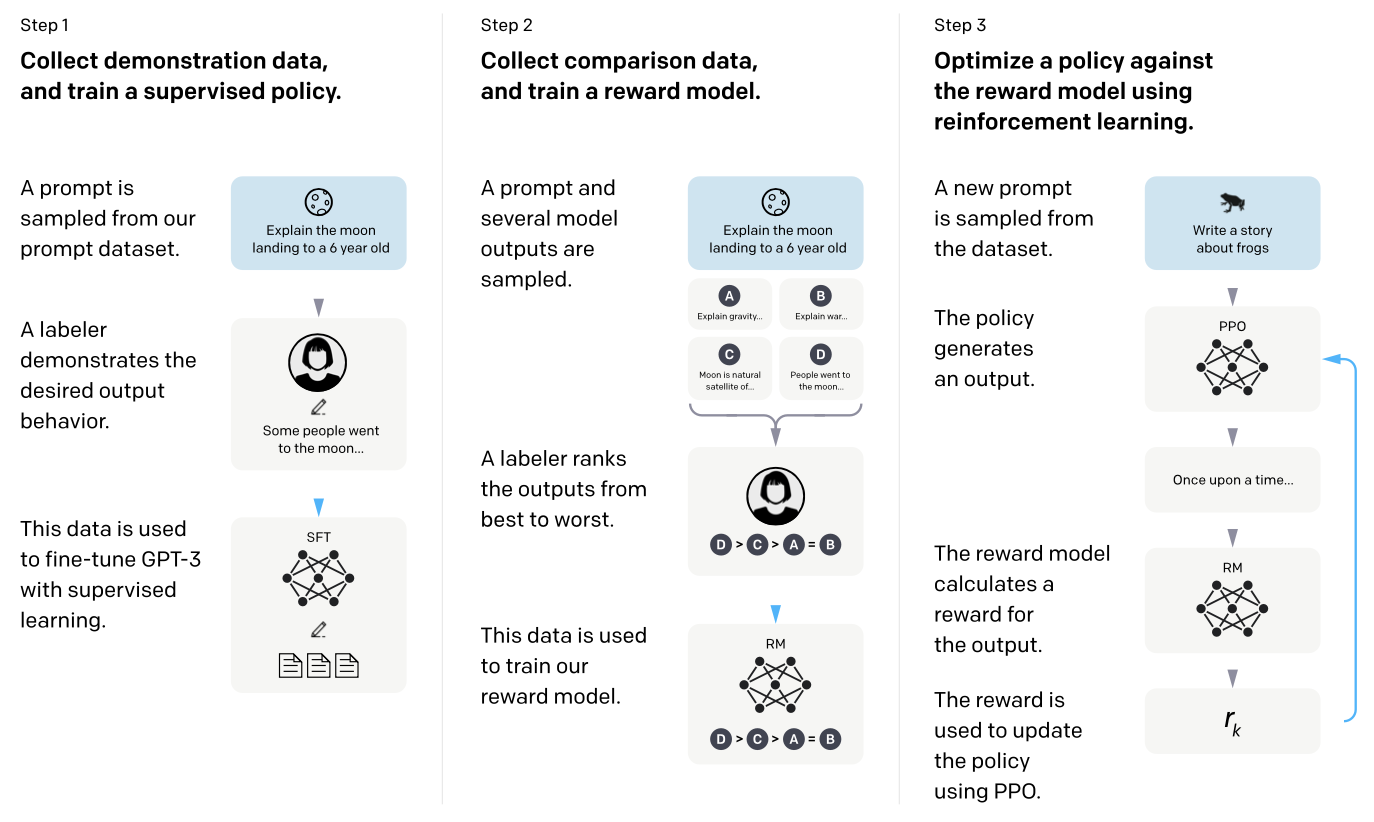
\includegraphics[scale=0.5]{images/ouyang2022_finetune_steps.png}
  \caption{Processo de ajuste fino. Fonte: \cite{ouyang2022}.}
  \label{fig:ouyang2022_finetuning}
\end{figure}

Operacionalmente, o SFT segue a lógica fundamental do pré-treinamento, utilizando a predição do próximo \textit{token} para internalizar informações de novos documentos \cite{ouyang2022}. A distinção reside no ponto de partida e na especificidade dos dados: enquanto o modelo base inicia com parâmetros aleatórios expostos a volumes massivos de dados genéricos, o SFT reutiliza os pesos pré-treinados, ajustando-os via gradiente descendente em conjuntos altamente curados. Essa reutilização permite que o modelo retenha o conhecimento linguístico geral enquanto assimila nuances e formatos especializados \cite{raff2025}.

\begin{figure}[htb]
  \centering
  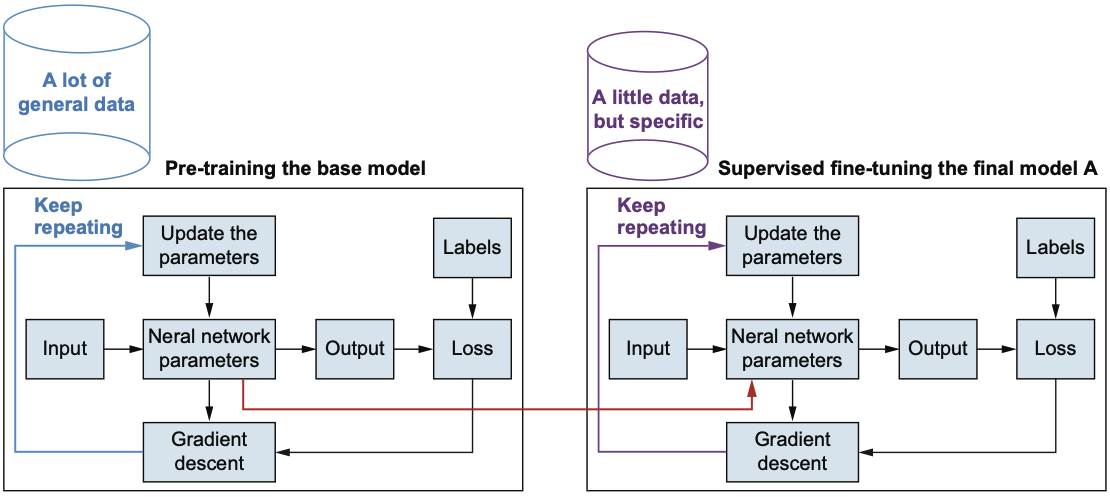
\includegraphics[scale=0.3]{images/raff2025_sft.png}
  \caption{O Supervised Fine-Tuning (SFT) como extensão do treinamento do modelo base em conjuntos de dados especializados. Fonte: \cite{raff2025}.}
  \label{fig:raff2025_sft}
\end{figure}

Entretanto, o ajuste fino impõe desafios intrínsecos, notadamente o esquecimento catastrófico (\textit{catastrophic forgetting}), onde a otimização para novas informações degrada a capacidade de processar dados anteriores \cite{ouyang2022}. Adicionalmente, objetivos abstratos — como a satisfação do usuário ou a segurança do conteúdo — são difíceis de alcançar exclusivamente com SFT. Para mitigar tais limitações, o RLHF (que compreende as duas últimas etapas do processo) introduz um modelo de recompensa que simula o julgamento humano, equilibrando a otimização da nova política com uma penalidade de similaridade em relação ao modelo original. Esse mecanismo de "objetivo duplo" assegura a evolução para atender às diretrizes sem degenerar em saídas incoerentes ou perder a naturalidade linguística conquistada no pré-treinamento \cite{raff2025}.

\begin{figure}[htb]
  \centering
  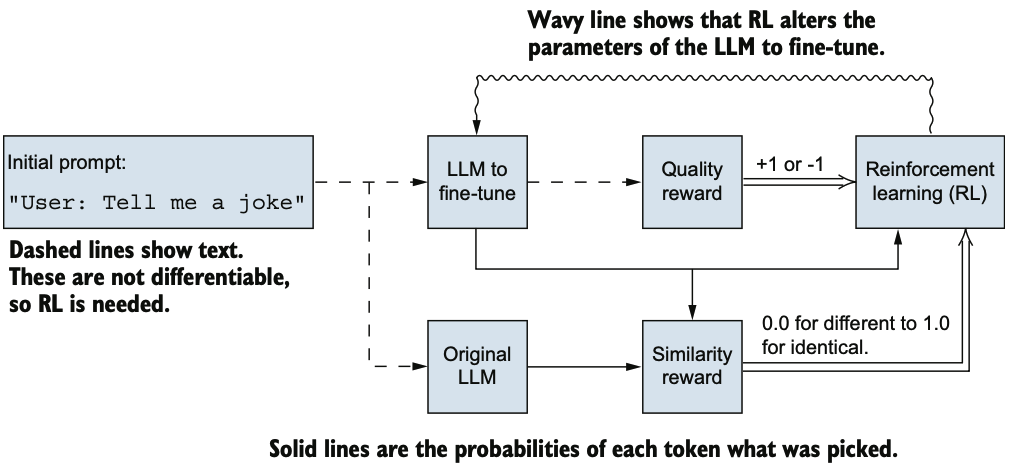
\includegraphics[scale=0.3]{images/raff2025_rlhf.png}
  \caption{RLHF: o aprendizado por reforço ajusta os parâmetros combinando pontuações de qualidade e similaridade para otimizar as saídas. Fonte: \cite{raff2025}.}
  \label{fig:raff2025_rlhf}
\end{figure}

Expande-se o escopo do ajuste fino através do \textit{Instruction Tuning}, abordagem que ajusta o modelo para uma diversidade de tarefas, aprimorando sua resposta em cenários \textit{zero-shot} \cite{wei2022finetune}. Essa metodologia utiliza uma mistura massiva de tarefas (tradução, raciocínio, análise de sentimentos) verbalizadas via \textit{templates} de linguagem natural. O objetivo é ensinar o modelo a generalizar o conceito de "seguir instruções" para tarefas inéditas, superando a limitação de apenas completar texto. Isso marca uma transição do aprendizado guiado por exemplos (\textit{example-driven}) para o guiado por instruções (\textit{instruction-driven}), onde as instruções atuam como supervisão indireta, permitindo ao modelo interpretar a intenção da tarefa sem depender de exemplos rotulados específicos \cite{lou2024}.

A eficácia dessa abordagem generalista depende criticamente da escala do modelo. Observa-se que, enquanto o ajuste de instruções potencializa a generalização em LLMs com mais de 68 bilhões de parâmetros, ele pode, paradoxalmente, degradar o desempenho de modelos menores em tarefas desconhecidas \cite{wei2022finetune}. Essa disparidade sugere que, se os grandes modelos operam como generalistas robustos, os SLMs beneficiam-se predominantemente de uma estratégia de "especialistas", na qual o ajuste é direcionado a domínios de interesse específicos \cite{wei2022finetune}.

A literatura indica, todavia, que o ajuste de instruções é vital para "desbloquear" capacidades latentes em arquiteturas menores, permitindo que estas superem versões significativamente maiores não refinadas \cite{zhao2025}. Evidências desse fenômeno surgem em modelos a partir de 77 milhões de parâmetros, com destaque para o Flan-T5 (11B), que superou o GPT-3 (175B) em 20 de 25 \textit{datasets} e ultrapassou o PaLM (62B) ao integrar dados de raciocínio \cite{wei2022finetune, chung2024}. Outro exemplo emblemático é o Med-PaLM, que atingiu performance comparável à de especialistas humanos ao refinar o modelo generalista com dados médicos \cite{zhao2025}. Assim, modelos menores ajustados para tarefas delimitadas — como \textit{tool calling} — conseguem igualar a eficácia de modelos massivos, oferecendo vantagens em latência e custo operacional \cite{belcak2025}.

Visando a viabilidade computacional, desenvolveram-se técnicas de ajuste fino com eficiência paramétrica (\textit{Parameter-Efficient Fine-Tuning} - PEFT). Dentre estas, o \textit{LoRA (Low-Rank Adaptation)} destaca-se por permitir a adaptação de modelos massivos sem a atualização de todos os seus parâmetros. A premissa baseia-se na hipótese de que a mudança nos pesos durante o ajuste possui uma "dimensão intrínseca" baixa \cite{hu2022}. Na prática, em vez de atualizar a matriz de pesos original $W \in \mathbb{R}^{d \times k}$, o LoRA congela $W$ e injeta duas matrizes de decomposição de baixa ordem, $A$ e $B$. Durante o treinamento, apenas essas matrizes menores são atualizadas, conforme a Equação \ref{eq:lora}:

\begin{equation}\label{eq:lora}
  h = W_0x + \Delta Wx = W_0x + BAx
\end{equation}

Onde $B \in \mathbb{R}^{d \times r}$, $A \in \mathbb{R}^{r \times k}$ e o \textit{rank} $r \ll \min(d,k)$ \cite{hu2022}. Essa abordagem reduz o número de parâmetros treináveis em até 10.000 vezes e a exigência de memória de GPU em 3 vezes para modelos como o GPT-3, sem introduzir latência adicional na inferência, visto que as matrizes podem ser fundidas aos pesos originais posteriormente \cite{hu2022}.

\begin{figure}[htb]
  \centering
  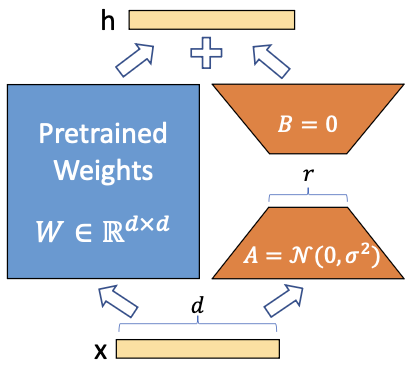
\includegraphics[scale=0.5]{images/hu2022_lora.png}
  \caption{Representação da técnica LoRA. Fonte: \cite{hu2022}.}
  \label{fig:hu2022_lora}
\end{figure}

O \textit{QLoRA (Quantized LoRA)} evolui esse conceito para reduzir ainda mais o uso de memória, viabilizando o ajuste de um modelo de 65B parâmetros em uma única GPU de 48GB \cite{dettmers2023}. O método opera através da retropropagação de gradientes por um modelo pré-treinado quantizado em 4 bits para os adaptadores LoRA, sustentado por três mecanismos centrais \cite{dettmers2023}:

\begin{itemize}
  \item \textbf{4-bit NormalFloat (NF4):} Preserva a precisão dos pesos melhor do que a quantização convencional.
  \item \textbf{Double Quantization:} Reduz o consumo de memória ao quantizar as próprias constantes de quantização.
  \item \textbf{Paged Optimizers:} Gerencia picos de memória durante o processamento para evitar erros de execução.
\end{itemize}

\begin{figure}[htb]
  \centering
  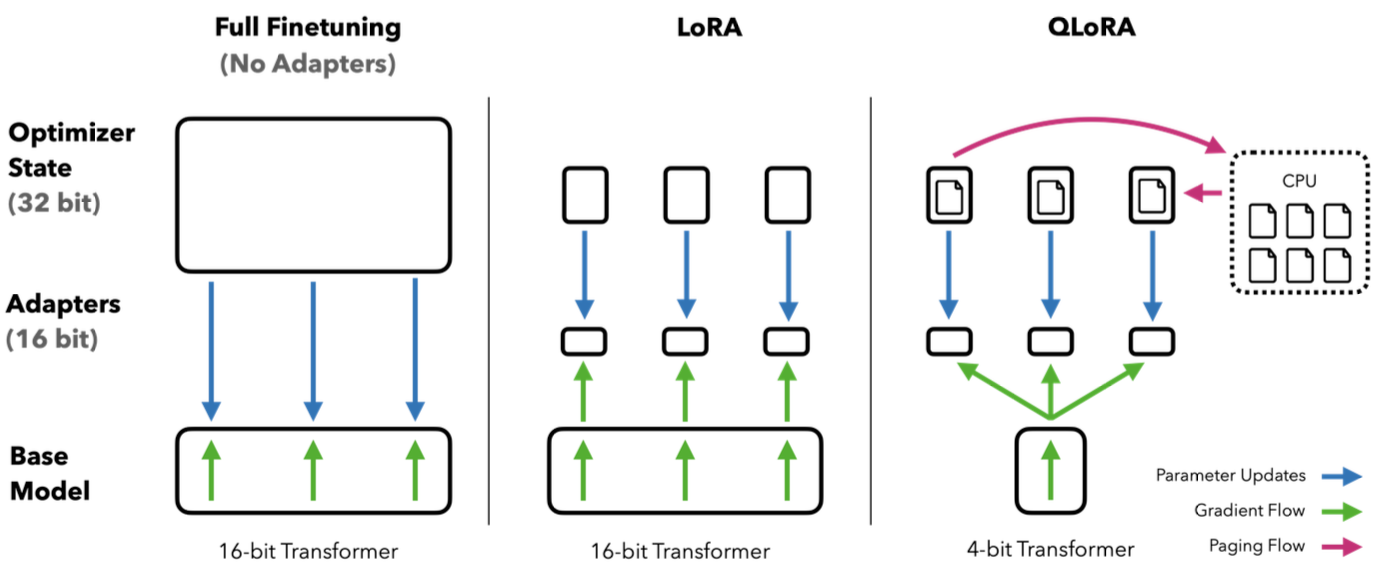
\includegraphics[scale=0.5]{images/dettmers2023_qlora.png}
  \caption{Comparação de métodos: QLoRA aprimora o LoRA via quantização de 4 bits e otimizadores paginados. Fonte: \cite{dettmers2023}.}
  \label{fig:dettmers2023_qlora}
\end{figure}

O sucesso do QLoRA é evidenciado pela família Guanaco, que atingiu 99,3\% do desempenho do ChatGPT no \textit{benchmark} Vicuna, exigindo apenas 24 horas de ajuste fino em uma única GPU profissional \cite{dettmers2023}.

\section{Sistemas de Agentes de Inteligência Artificial}

Um agente de IA define-se como um sistema computacional capaz de perceber seu ambiente, raciocinar e executar ações para alcançar objetivos \cite{russel2020}. Para concretizar tais propósitos, essa entidade assume o papel de um agente racional: aquele que, para cada sequência de percepções, seleciona a ação que maximiza sua medida de desempenho esperada, ponderando as evidências perceptivas e o conhecimento prévio acumulado \cite{russel2020}. O conceito estrutura-se em quatro componentes fundamentais:

\begin{itemize}
  \item \textit{Medida de Desempenho (Performance Measure):} critério objetivo para avaliar o sucesso do comportamento do agente. Constitui a métrica que qualifica a sequência de estados no ambiente, gerada pelas ações do agente, como desejável ou indesejável \cite{russel2020}.
  \item \textit{Ambiente (Environment):} contexto externo de operação. A natureza deste meio (total ou parcialmente observável, determinístico ou estocástico, estático ou dinâmico) determina a complexidade do design do sistema \cite{russel2020}.
  \item \textit{Atuadores (Actuators):} mecanismos pelos quais o agente influencia ou altera o ambiente. Representam os meios de execução das ações selecionadas pelo programa do agente \cite{russel2020}.
  \item \textit{Sensores (Sensors):} dispositivos ou métodos que permitem a recepção de informações sobre o estado atual do ambiente e o estado interno do sistema \cite{russel2020}.
\end{itemize}

O programa do agente rege a relação entre esses componentes, implementando a função que mapeia o histórico de percepções em ações. Tradicionalmente baseados em regras simbólicas ou lógica formal \cite{russel2020}, o paradigma recente direcionou o foco para agentes fundamentados em LLMs \cite{kong2024, yao2023}. Inicialmente, explorou-se a capacidade de raciocínio desses modelos via \textit{Chain-of-Thought} (CoT), induzindo a verbalização de passos intermediários para resolução de problemas complexos, o que sugeriu o uso de LLMs como o "cérebro" do agente. Contudo, o CoT, ao depender exclusivamente de representações internas, opera como uma "caixa estática", suscetível a alucinações e propagação de erros por falta de ancoragem no mundo externo \cite{wei2022cot}.

Nesse cenário, o paradigma ReAct (\textit{Reason + Act}) propõe uma evolução arquitetural significativa. O método transcende as limitações do CoT ao sinergizar o raciocínio verbal com a tomada de decisão sequencial. Enquanto o CoT provê o planejamento e decomposição de metas (componente \textit{Reason}), o ReAct integra a interação com o ambiente (componente \textit{Act}) para validação. Sob uma perspectiva formal, o ReAct expande o espaço de ação tradicional: dado um sistema onde, no passo $t$, o agente recebe uma observação $o_{t} \in \mathcal{O}$ e executa uma ação $a_{t} \in \mathcal{A}$ seguindo uma política $\pi(a_{t}|c_{t})$, o espaço de ação é aumentado para $\hat{\mathcal{A}} = \mathcal{A} \cup \mathcal{L}$, onde $\mathcal{L}$ denota o espaço da linguagem \cite{yao2023}.

Nesse espaço aumentado, define-se uma ação $\hat{a}_{t} \in \mathcal{L}$ como um \textit{pensamento} ou \textit{traço de raciocínio}. Diferentemente das ações físicas ($\mathcal{A}$), o pensamento não afeta o ambiente externo nem gera \textit{feedback} imediato. Sua função consiste em compor informações úteis raciocinando sobre o contexto atual $c_{t}$, atualizando-o para $c_{t+1} = (c_{t}, \hat{a}_{t})$ de modo a influenciar as decisões subsequentes \cite{yao2023}.

Essa arquitetura viabiliza um funcionamento dinâmico cíclico em duas modalidades:
\begin{enumerate}
  \item \textit{Raciocinar para Agir (Reason to Act):} emprego de traços de raciocínio para criar, manter e ajustar planos de alto nível dinamicamente, tratando exceções antes da execução física \cite{yao2023}.
  \item \textit{Agir para Raciocinar (Act to Reason):} interação com interfaces externas (APIs, ambientes virtuais) para coletar informações adicionais que fundamentem o raciocínio em fatos observados \cite{yao2023}.
\end{enumerate}

Essa alternância contrasta com métodos de planejamento estático ou puramente reativos. Enquanto modelos \textit{Act-Only} limitam-se no rastreamento de estados complexos e modelos \textit{Reason-Only} (como o CoT) permanecem propensos a alucinações, a intercalação entre a geração de pensamentos ($\hat{a}_{t} \in \mathcal{L}$) e ações no ambiente ($a_{t} \in \mathcal{A}$) resulta em trajetórias de solução viáveis e factualmente ancoradas \cite{yao2023}.

A execução robusta da etapa de "Agir" ($a_{t} \in \mathcal{A}$) demanda a mitigação das limitações intrínsecas aos modelos probabilísticos, notadamente a falta de acesso a dados dinâmicos e a falibilidade em cálculos exatos. A arquitetura MRKL (\textit{Modular Reasoning, Knowledge and Language}) formaliza uma abordagem neuro-simbólica que endereça essas deficiências ao desacoplar o processamento linguístico da execução de tarefas \cite{karpas2022}.

Neste modelo, o sistema opera via uma composição de módulos governada por um \textit{Roteador} neural e um conjunto de \textit{Especialistas} \cite{karpas2022}. O papel do modelo de linguagem desloca-se da geração de respostas finais para o controle de fluxo, redefinindo a arquitetura em três pontos centrais:

\begin{itemize}
  \item \textit{Seleção de Módulos:} o Roteador analisa a entrada em linguagem natural para identificar a intenção e selecionar o especialista adequado (modelo neural ou motor simbólico, como calculadoras ou APIs) \cite{karpas2022}.
  \item \textit{Extração de Parâmetros:} o modelo extrai do texto argumentos discretos necessários para a chamada da função, atuando como interface semântica para sistemas determinísticos \cite{karpas2022}.
  \item \textit{Extensibilidade Robusta:} o espaço de ação expande-se para incluir operações externas, permitindo adicionar capacidades sem retreino do modelo base, transpondo o abismo entre processamento probabilístico e raciocínio exato \cite{karpas2022}.
\end{itemize}

Enquanto a arquitetura MRKL formaliza a separação entre raciocínio neural e execução simbólica via roteadores, desenvolvimentos recentes buscam integrar o \textit{tool calling} diretamente nos pesos do modelo, tratando o uso de ferramentas como extensão nativa da modelagem de linguagem \cite{schick2023,parisi2022}.

Conforme ilustrado na Figura \ref{fig:parisi2022_talm}, a definição de \textit{tool calling} é formalizada através de uma interface \textit{text-to-text} agnóstica à arquitetura \cite{parisi2022}. O fluxo de execução converte-se em uma sequência contínua de \textit{tokens}: dado um \texttt{input} de tarefa, o modelo gera um \texttt{tool input} seguido por um delimitador; a ferramenta processa a entrada e anexa o \texttt{tool result} à sequência; finalmente, o modelo atende a esse histórico aumentado para gerar o \texttt{output} final \cite{parisi2022}.

\begin{figure}[htb]
  \centering
  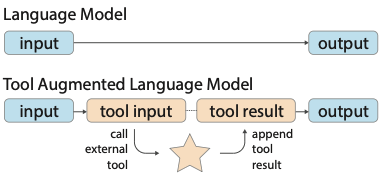
\includegraphics[scale=0.6]{images/parisi2022_talm.png}
  \caption{Arquitetura TALM (\textit{Tool-Augmented Language Models}): ciclo de interação entre modelo e ferramentas via interface de texto. Fonte: \cite{parisi2022}.}
  \label{fig:parisi2022_talm}
\end{figure}

O experimento \textit{Toolformer} abordou a autonomia de LLMs no uso de ferramentas (calculadoras, tradutores, APIs) \cite{schick2023}. A inovação central residiu na inserção de chamadas de API diretamente no texto de treino. Por exemplo, a sentença "O Joe Biden nasceu em Scranton" transforma-se em "O Joe Biden nasceu em \texttt{[Search(Joe Biden birth place)]} Scranton". Este trabalho fundamenta o atual "Function Calling" em modelos comerciais, evidenciando como a preparação do \textit{dataset} permite que o modelo aprenda a orquestrar sistemas externos \cite{schick2023}.

Nesse modelo, a chamada de ferramenta é representada linearmente como $c=(a_c, i_c)$, onde $a_c$ é o nome da API e $i_c$ a entrada, encapsulada por \textit{tokens} especiais. Tal competência pode ser aprendida via SFT e ajuste fino, eliminando a necessidade de anotação humana massiva mediante um ciclo auto-supervisionado: o modelo amostra e executa chamadas, filtrando e retreinando apenas naquelas que reduzem a perplexidade da predição subsequente \cite{parisi2022}. Essa convergência de métodos concretiza a visão neuro-simbólica ponta-a-ponta, materializando agentes de IA que utilizam ferramentas para atingir objetivos a partir da observação do ambiente \cite{parisi2022, schick2023, kong2024}.

Sistemas inteligentes complexos emergem da combinação de agentes de IA cujas interações visam um objetivo comum \cite{hulten2018}. A comunicação pode ser colaborativa — onde agentes cooperam para metas compartilhadas inatingíveis individualmente — ou competitiva, onde um agente maximiza sua performance em detrimento de outros \cite{li2023, russel2020}.

Para abordar problemas complexos e simular cenários realistas, surgiram arquiteturas multiagentes baseadas em LLMs \cite{guo2024}. A adoção dessa arquitetura justifica-se pelo princípio da divisão do trabalho: tarefas complexas são decompostas em sub-rotinas atribuídas a agentes especializados \cite{xi2025}. Essa especialização mitiga problemas inerentes aos LLMs isolados, como alucinações e janela de contexto limitada, permitindo foco em domínios específicos. A interação pode seguir formatos estruturados, sequenciais, hierárquicos ou colaborativos (Figura \ref{fig:xi2025_types_of_agent_colaboration}), mimetizando equipes humanas \cite{xi2025}.

\begin{figure}[htb]
  \centering
  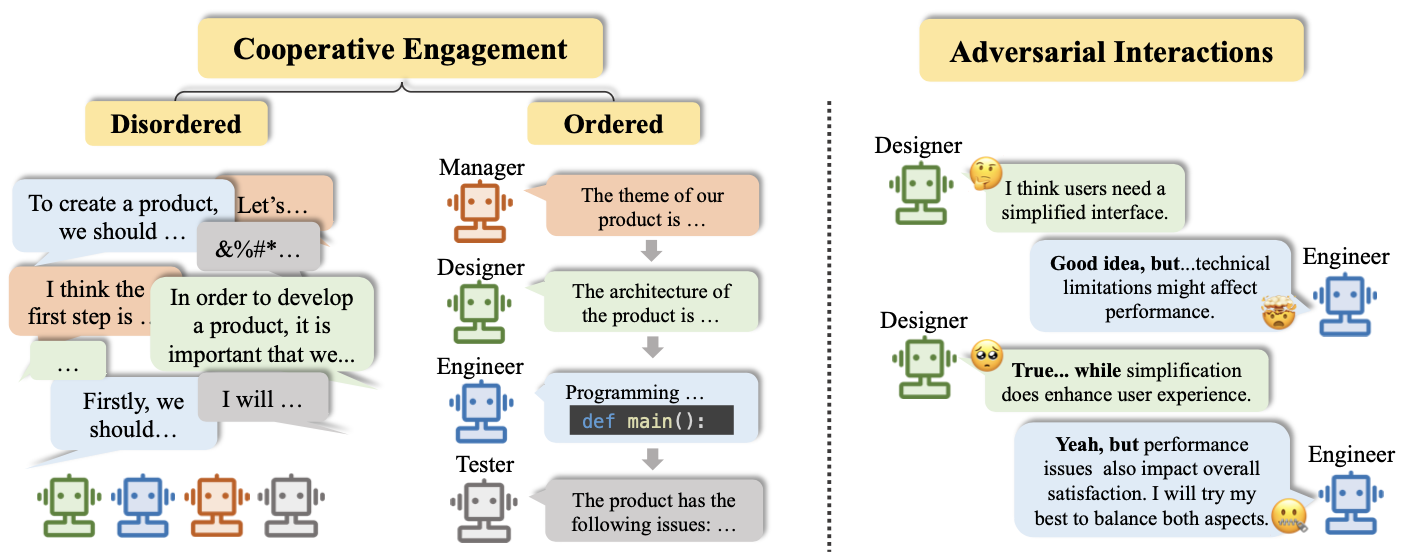
\includegraphics[scale=0.5]{images/xi2025_types_of_agent_colaboration.png}
  \caption{Cenários de Interação para Sistemas Multiagentes com LLMs. Fonte: \cite{xi2025}.}
  \label{fig:xi2025_types_of_agent_colaboration}
\end{figure}

A aplicação da divisão do trabalho reduz, ainda, a carga cognitiva exigida de um único modelo. Ao restringir o escopo de atuação, diminui-se a probabilidade de interferências de conhecimentos não relacionados \cite{xi2025}. Essa compartimentalização favorece SLMs que, embora possuam menos parâmetros, podem apresentar desempenho superior em tarefas verticais quando dotados de conhecimento de domínio \cite{belcak2025}. Tal desempenho observa-se em desenvolvimento de software, onde a simulação de papéis (gerentes, programadores, testadores) resulta em códigos mais robustos comparados àqueles gerados por agentes únicos \cite{guo2024}.

A operacionalização dessa colaboração autônoma ocorre em frameworks de interpretação de papéis, como o CAMEL. Nessa arquitetura, coopera-se entre um agente usuário (instruções de domínio) e um agente assistente (execução técnica), mediados por um especificador de tarefas. A avaliação quantitativa evidenciou que essa abordagem de diálogo corrige autonomamente desvios e alucinações, obtendo preferência em 76\% das avaliações humanas em tarefas de programação frente a agentes isolados \cite{li2023}.

Avançando na complexidade, o framework AutoGen possibilitou interações focadas tanto em colaboração quanto em orquestração \cite{wu2024}. O OptiGuide, uma de suas implementações, designa um agente "Comandante" para coordenar um "Escritor" (geração de código) e uma "Salvaguarda" (segurança) (Figura \ref{fig:wu2024_optiguide}). Diferente de cadeias lineares, o orquestrador mantém o contexto e decide dinamicamente quando invocar validação ou correções, criando um ciclo de \textit{feedback} autônomo que reduz a intervenção humana e aumenta a precisão do código \cite{wu2024}.

\begin{figure}[htb]
  \centering
  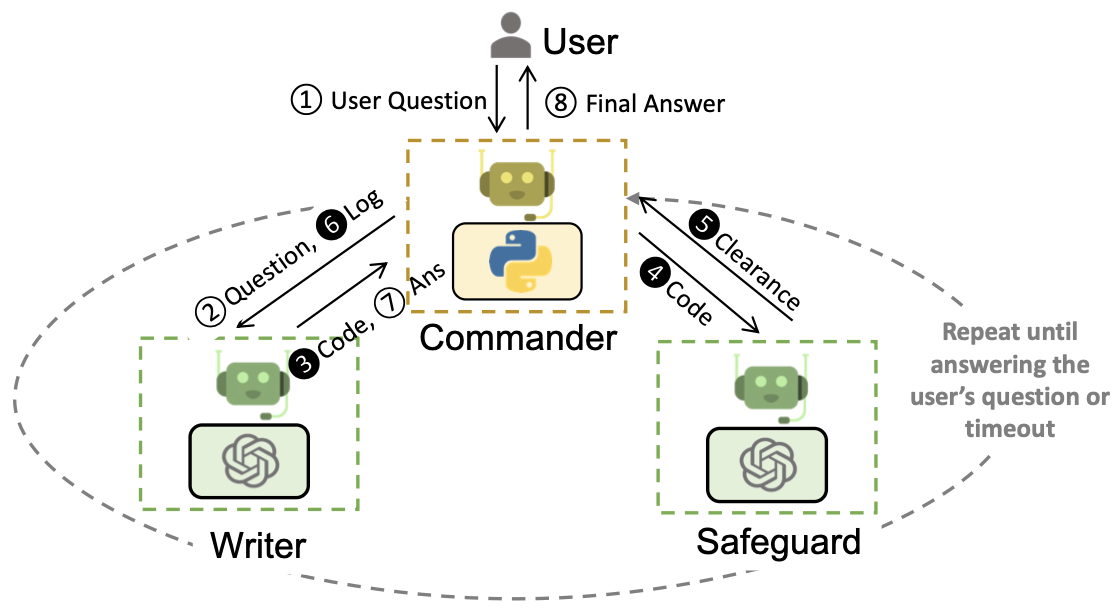
\includegraphics[scale=0.5]{images/wu2024_optiguide.png}
  \caption{Arquitetura multiagente no sistema OptiGuide: interação entre agentes de coordenação, escrita e salvaguarda. Fonte: \cite{wu2024}.}
  \label{fig:wu2024_optiguide}
\end{figure}

Em uma perspectiva de maior estruturação processual, o framework MetaGPT introduziu Procedimentos Operacionais Padrão (SOPs) em sistemas multiagentes, simulando fluxos corporativos \cite{hong2024}. Diferentemente de abordagens de chat livre, essa arquitetura impõe comunicação via saídas estruturadas (documentos de requisitos, diagramas). Ao atribuir papéis rígidos (Gerente de Produto, Arquiteto, Engenheiro, QA), o sistema mitiga a degradação da informação comum em diálogos longos.

A eficácia dessa metodologia reside no mecanismo de \textit{feedback} executável em tempo de execução, onde o agente de engenharia utiliza erros de compilação para ajustar o código iterativamente. Resultados nos benchmarks HumanEval e MBPP indicam taxas de sucesso superiores a 85\% na geração de código funcional, superando frameworks conversacionais \cite{hong2024}. A Figura \ref{fig:hong2024_metagpt_sop} ilustra a decomposição do fluxo em etapas sequenciais com entregáveis definidos.

\begin{figure}[htb]
  \centering
  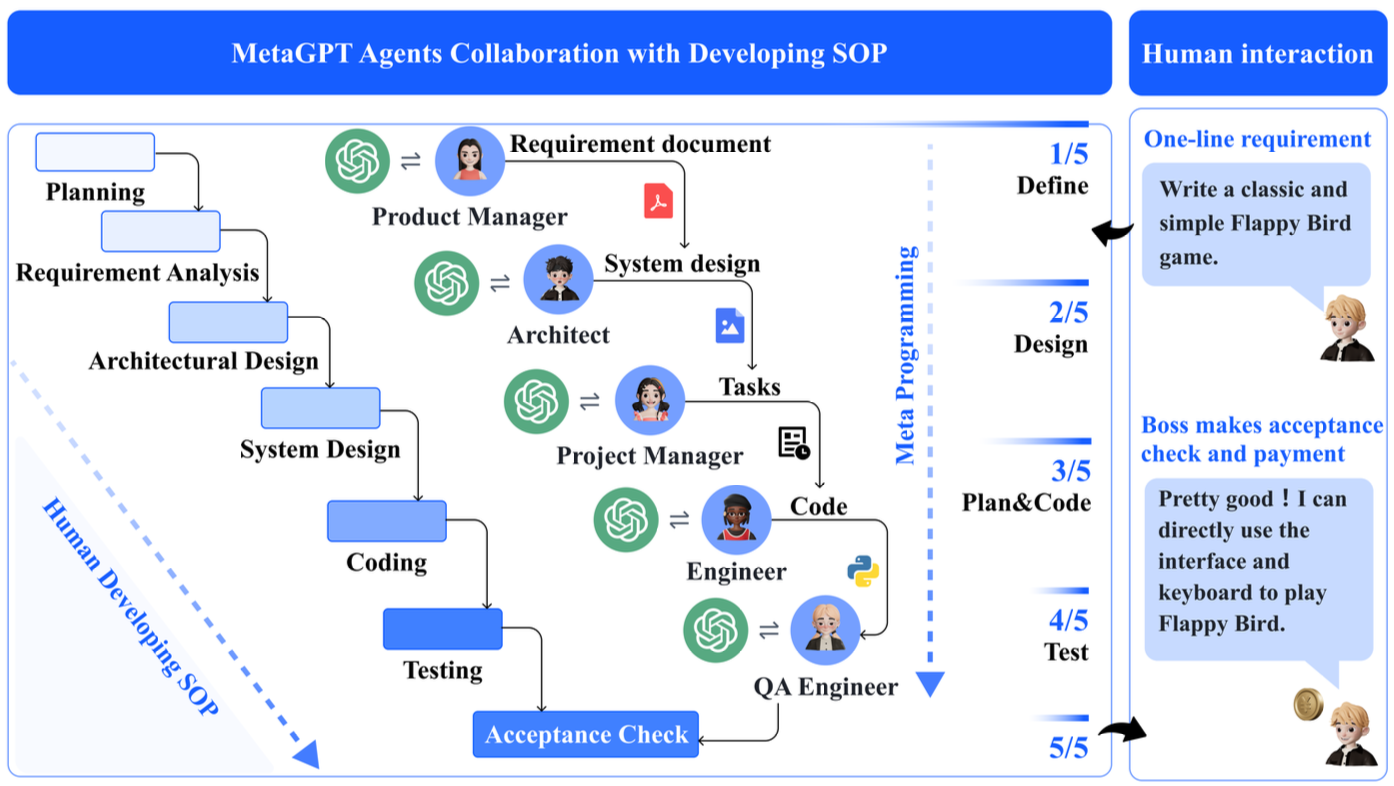
\includegraphics[scale=0.4]{images/hong2024_metagpt_sop.png}
  \caption{Fluxo de trabalho baseado em SOPs no MetaGPT. Fonte: \cite{hong2024}.}
  \label{fig:hong2024_metagpt_sop}
\end{figure}

Essa decomposição de tarefas estende-se a interfaces \textit{Text-to-SQL}, onde a complexidade envolve a compreensão de esquemas extensos. Arquiteturas colaborativas como o MAC-SQL estruturam o processo em três papéis: seleção, decomposição e refinamento \cite{wang2025macsql}. Um agente "Seletor" filtra o conhecimento de domínio, descartando tabelas irrelevantes para manter o foco na janela de contexto; um "Decompositor" fragmenta perguntas complexas; e um "Refinador" valida e corrige o SQL gerado via ferramentas externas \cite{wang2025macsql}. Testes com modelos de até 7B parâmetros ajustados demonstraram resultados comparáveis aos de LLMs generalistas, provando que a orquestração inteligente viabiliza o uso de SLMs em tarefas de alta complexidade semântica \cite{wang2025macsql}.

Ainda no contexto de especialização para SLMs, o framework MATS operacionaliza a verificação e correção iterativa baseada no retorno do banco de dados, dividindo a inferência em cinco papéis \cite{hoang2025}. O diferencial reside na introdução de agentes validadores especializados — focados em seleção de colunas e condições lógicas — que comparam a intenção da pergunta com a execução preliminar. Caso inconsistências sejam detectadas, aciona-se um agente de "Correção". O treinamento por reforço com \textit{feedback} de execução (RLE) permite que o sistema evolua e supere o desempenho de agentes isolados, mesmo utilizando modelos menores \cite{hoang2025}.

Apesar dos benefícios, sistemas multiagentes enfrentam desafios técnicos distintos, sendo a propagação de erros um dos mais críticos \cite{hulten2018}. Diferente da alucinação isolada em agente único, em arquiteturas colaborativas o fenômeno pode gerar um efeito cascata, onde a informação incorreta é assumida como verdadeira pelos agentes subsequentes. Isso evidencia a dependência do "elo mais fraco", desafio exacerbado ao utilizarem-se modelos menores e mais propensos a erros \cite{guo2024}.

A adoção de SLMs em arquiteturas multiagentes impõe, portanto, limites cognitivos específicos \cite{belcak2025}. Uma barreira significativa reside na hipótese de que apenas modelos de larga escala abstraem informações semânticas complexas de domínios variados. Pragmaticamente, essa restrição manifesta-se no planejamento: embora proficientes em tarefas procedurais e código rotineiro, SLMs enfrentam dificuldades substanciais em raciocínio arquitetural, planejamento adaptativo e resolução de erros não estruturados quando comparados a modelos generalistas \cite{belcak2025}.

\section{Interfaces Text-to-SQL}

As tarefas \textit{Text-to-SQL} constituem um subdomínio do campo de PLN e consistem na interpretação da linguagem natural para identificação de entidades e intenções, traduzindo-as para uma consulta estruturada executável e compatível com o esquema de um banco de dados em SQL \cite{quamar2022}. Historicamente, duas abordagens principais prevaleceram: sistemas baseados em regras e aqueles baseados em aprendizado de máquina ou profundo (\textit{Deep Learning}). Sistemas baseados em regras dependem de índices semânticos, ontologias e grafos de conhecimento, utilizando gramáticas para gerar as consultas. Já as abordagens baseadas em aprendizado profundo codificam a entrada do usuário para treinar modelos que geram a consulta SQL. Recentemente, a convergência para arquiteturas híbridas busca mitigar as limitações individuais de cada método \cite{quamar2022}.

Os desafios na consulta em linguagem natural dividem-se em três tarefas fundamentais: (1) identificar as entidades no texto do usuário; (2) conectar tais entidades à fonte de dados para interpretar intenções; e (3) gerar a consulta estruturada final \cite{quamar2022}. A análise semântica e a marcação de entidades focam nos termos relevantes, mas a etapa seguinte é a mais crítica, pois exige o mapeamento desses elementos para o esquema do banco de dados a fim de decifrar a intenção do usuário sob ambiguidades complexas. Por fim, a tradução concretiza a interpretação em linguagem de consulta \cite{quamar2022}. A democratização do acesso aos dados motiva essas interfaces, oferecendo um mecanismo para que usuários não técnicos investiguem conjuntos de dados sem dominar linguagens complexas \cite{shi2025}. Na indústria, essa acessibilidade reduz a dependência de equipes técnicas e a latência na tomada de decisão, transformando o gestor em um "consumidor aumentado" \cite{quamar2022}.

A evolução dos LLMs alterou o paradigma de desenvolvimento dessas interfaces para arquiteturas híbridas, transitando de modelos heterogêneos e específicos para uma base unificada em \textit{Transformers} (Figura \ref{fig:shi2025_llms_in_text_to_sql}).

\begin{figure}[htb]
  \begin{center}
    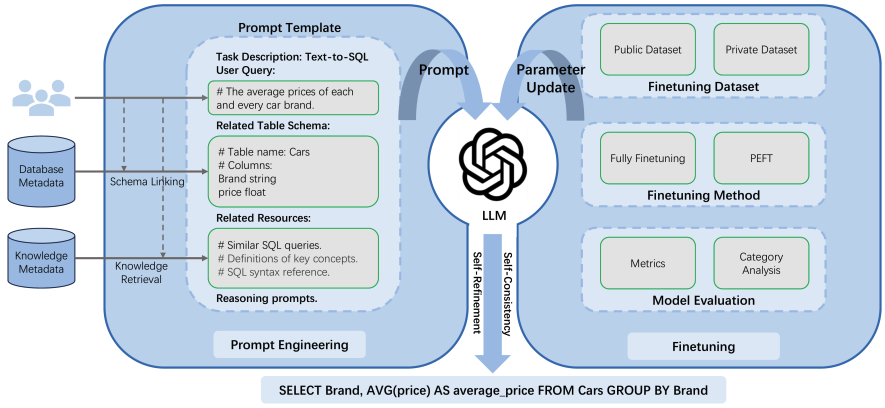
\includegraphics[scale=0.5]{images/shi2025_llms_in_text_to_sql.png}
  \end{center}
  \caption{\label{fig:shi2025_llms_in_text_to_sql}Framework de LLMs em Text-to-SQL. (Fonte: \citeonline{shi2025})}
\end{figure}

Atualmente, a aplicação de LLMs em \textit{Text-to-SQL} divide-se em duas vertentes: engenharia de \textit{prompt} — com técnicas como \textit{Retrieval-Augmented Generation} (RAG), \textit{Chain-of-Thought}, \textit{Few-Shot Learning} e \textit{Tool Calling} \cite{wang2025llmsurvey, wei2022cot, parisi2022} — e \textit{fine-tuning}, focado na especialização do modelo e eficiência de parâmetros \cite{ouyang2022, shi2025}. Essa mudança arquitetural resultou em um salto qualitativo na acurácia em \textit{benchmarks} consolidados, estabelecendo o novo estado da arte \cite{shi2025}.

O impacto disruptivo dessas tecnologias permite dividir os \textit{datasets} de treinamento e avaliação em "pré-LLMs" e "pós-LLMs" \cite{shi2025}. \textit{Benchmarks} anteriores, como WikiSQL e, notadamente, o Spider \citeonline{yu2018}, focavam na análise semântica em domínios cruzados e na correspondência estrutural exata. Com a ascensão dos LLMs, surgiram métricas para mensurar capacidades emergentes e desafios corporativos reais, como o uso de conhecimento de domínio, manipulação de esquemas massivos e robustez contra ruídos, destacando-se o BIRD e o CoSQL. Contudo, o Spider permanece como a principal escolha para avaliar performance de tarefas \textit{Text-to-SQL} \cite{shi2025}.

Tradicionalmente, a avaliação baseia-se na Correspondência Exata (\textit{Exact Set Match Accuracy} - EM) e na Acurácia de Execução (\textit{Execution Accuracy} - EX) \cite{yu2018, shi2025}. A EM verifica se a consulta gerada é idêntica à de referência em componentes estruturais, sem considerar a execução \cite{ascoli2025}. No entanto, essa métrica tende a subestimar a capacidade do modelo com falsos negativos, pois penaliza variações sintáticas válidas, como a equivalência semântica entre a função \texttt{MAX} e uma ordenação seguida de \texttt{LIMIT 1} (Figura \ref{fig:ascoli2025_ex_example}) \cite{ascoli2025}.

\begin{figure}[htb]
  \begin{center}
    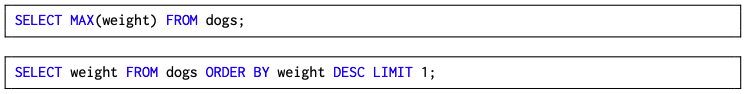
\includegraphics[scale=0.6]{images/ascoli2025_ex_example.png}
  \end{center}
  \caption{\label{fig:ascoli2025_ex_example}Exemplo de falso negativo na métrica EM. As consultas buscam o peso máximo de formas distintas, levando a EM a classificar a geração como incorreta. (Fonte: \citeonline{ascoli2025})}
\end{figure}

Por outro lado, a EX avalia a correção funcional ao comparar os resultados da execução \cite{yu2018}. Embora pragmática, ela é suscetível a superestimar o desempenho (falsos positivos) quando consultas logicamente distintas retornam o mesmo resultado devido ao estado momentâneo do banco de dados (Figura \ref{fig:ascoli2025_em_example}) \cite{shi2025}. Em modelos não submetidos a ajuste fino, a taxa de falsos positivos da EX pode chegar a 23,0\% \cite{ascoli2025}.

\begin{figure}[htb]
  \begin{center}
    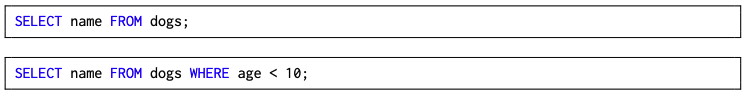
\includegraphics[scale=0.6]{images/ascoli2025_em_example.png}
  \end{center}
  \caption{\label{fig:ascoli2025_em_example}Exemplo de falso positivo na métrica EX. O filtro extra altera a semântica, mas retorna o mesmo resultado vazio, gerando uma classificação incorreta de acerto. (Fonte: \citeonline{ascoli2025})}
\end{figure}

Para mitigar tais limitações, a literatura recente propõe a \textit{Enhanced Tree Matching} (ETM), que avalia a equivalência semântica comparando a Árvore Sintática Abstrata (AST) das consultas \cite{ascoli2025}. O método aplica regras de normalização para formas canônicas e valida restrições de esquema (chaves primárias e unicidade), reduzindo as taxas de erro de avaliação para níveis inferiores a 3\% \cite{ascoli2025}.

Diante do novo paradigma de performance, as abordagens abandonam a geração monolítica em favor de estruturas decompostas e especializadas. Estratégias focadas na engenharia de fluxo de raciocínio, como o DIN-SQL \cite{pourreza2023} e o DAIL-SQL \cite{gao2024}, fundamentam-se na premissa de que a capacidade de raciocínio dos LLMs é ampliada ao fragmentar o problema em sub-tarefas menores \cite{pourreza2023}. O DIN-SQL (\textit{Decomposed In-Context Learning}) estrutura o processo em quatro módulos: vinculação de esquema (\textit{schema linking}); classificação e decomposição da consulta; geração baseada na complexidade; e autocorreção (\textit{self-correction}) \cite{pourreza2023}. Essa arquitetura demonstra que a decomposição permite que modelos generalistas superem modelos com \textit{fine-tuning} extensivo em diversos \textit{benchmarks} \cite{pourreza2023}.

\begin{figure}[htb]
  \begin{center}
    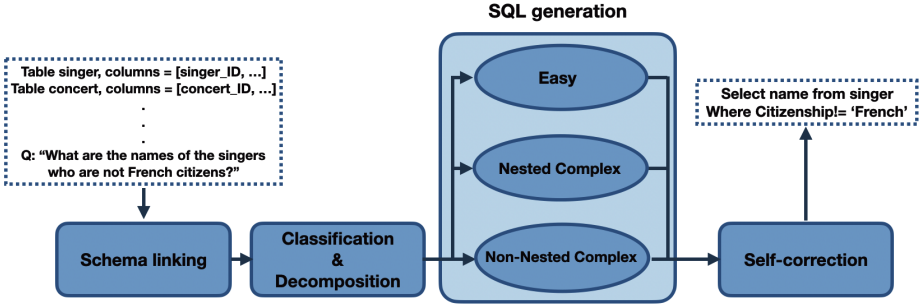
\includegraphics[scale=0.3]{images/pourreza2023_din_sql.png}
  \end{center}
  \caption{\label{fig:pourreza2023_din_sql}Arquitetura do DIN-SQL. (Fonte: \citeonline{pourreza2023})}
\end{figure}

O DAIL-SQL (\textit{Data Augmentation and Interaction Learning for SQL}) prioriza a eficiência de \textit{tokens} e a seleção criteriosa de exemplos, assumindo que a qualidade dos casos no cenário \textit{few-shot} e a representação do esquema são determinantes \cite{gao2024}. O método introduz o \textit{DAIL Selection}, que considera as similaridades semântica e estrutural das consultas. Além disso, valida-se a superioridade do uso de \textit{Code Representation Prompts} (CR) via comandos DDL (\texttt{CREATE TABLE}), aproveitando o pré-treinamento dos modelos em código \cite{gao2024}.

Entretanto, a aplicação dessas técnicas de \textit{prompting} em SLMs apresenta restrições. Modelos da família LLaMA e Vicuna, em seu estado base, possuem capacidade de raciocínio inferior aos modelos proprietários. Embora o \textit{Supervised Fine-Tuning} (SFT) eleve a performance desses SLMs, observa-se o efeito colateral de degradação da capacidade de \textit{In-Context Learning}: após o ajuste, os modelos tendem a perder a habilidade de generalizar a partir de exemplos fornecidos no contexto, evidenciando que a adaptação de SLMs exige mais do que apenas treinamento em \textit{datasets} genéricos \cite{gao2024}.

Nesse cenário, o framework CodeS especializa o uso de SLMs para mitigar as restrições de janela de contexto. A arquitetura integra módulos de pré-processamento para otimizar a entrada: um Filtro de Esquema e um Recuperador de Valores (\textit{Value Retriever}) via índices BM25 \cite{li2024}.

\begin{figure}[htb]
  \begin{center}
    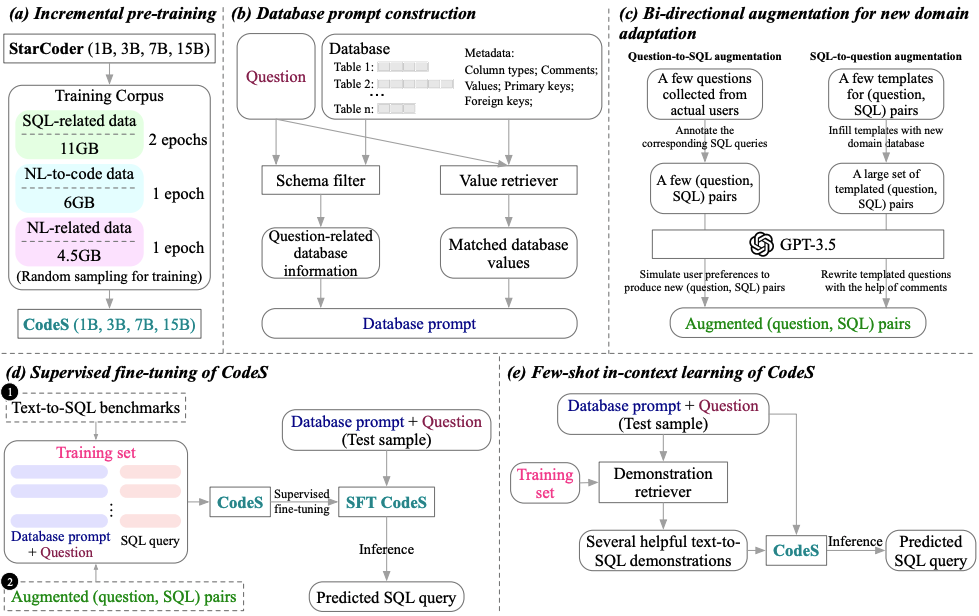
\includegraphics[scale=0.3]{images/li2024_codes.png}
  \end{center}
  \caption{\label{fig:li2024_codes}Arquitetura do CodeS. (Fonte: \citeonline{li2024})}
\end{figure}

Essa redução de dimensionalidade, combinada ao pré-treinamento incremental em SQL, permite que modelos com 3B ou 7B de parâmetros superem LLMs massivos em robustez e execução \cite{li2024}. Corroborando essa viabilidade, o framework DB-GPT-Hub \cite{zhou2024} demonstra que técnicas de eficiência de parâmetros (PEFT), como LoRA e QLoRA, permitem que SLMs alcancem desempenho comparável a modelos base significativamente maiores operando apenas via \textit{prompting} \cite{zhou2024}. Todavia, os ganhos do ajuste fino possuem correlação negativa com a complexidade da consulta: embora eficazes em tarefas simples e médias, a margem de ganho estreita-se em cenários complexos (Figura \ref{fig:zhou2024_improvement}) \cite{zhou2024}. Isso sugere que a especialização alinha o modelo à sintaxe, mas é insuficiente para prover a lógica de raciocínio necessária para aninhamentos e junções múltiplas.

\begin{figure}[htb]
  \begin{center}
    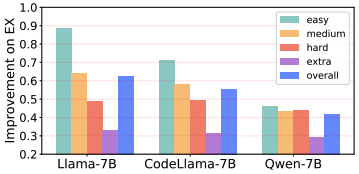
\includegraphics[scale=0.7]{images/zhou2024_improvement.png}
  \end{center}
  \caption{\label{fig:zhou2024_improvement}Melhoria de desempenho (EX) obtida com LoRA. O ganho é menor em tarefas de alta complexidade. (Fonte: \citeonline{zhou2024})}
\end{figure}

Para superar esse gargalo, a literatura recente propõe Sistemas Multiagentes (SMA), como o MAC-SQL \cite{wang2025macsql}, onde a responsabilidade da geração é distribuída entre unidades funcionais: um \textit{Selector}, que mitiga ruído no esquema; um \textit{Decomposer}, que fragmenta a pergunta via \textit{Chain-of-Thought}; e um \textit{Refiner}, que corrige erros com base no retorno do banco de dados \cite{wang2025macsql}.

\begin{figure}[htb]
  \begin{center}
    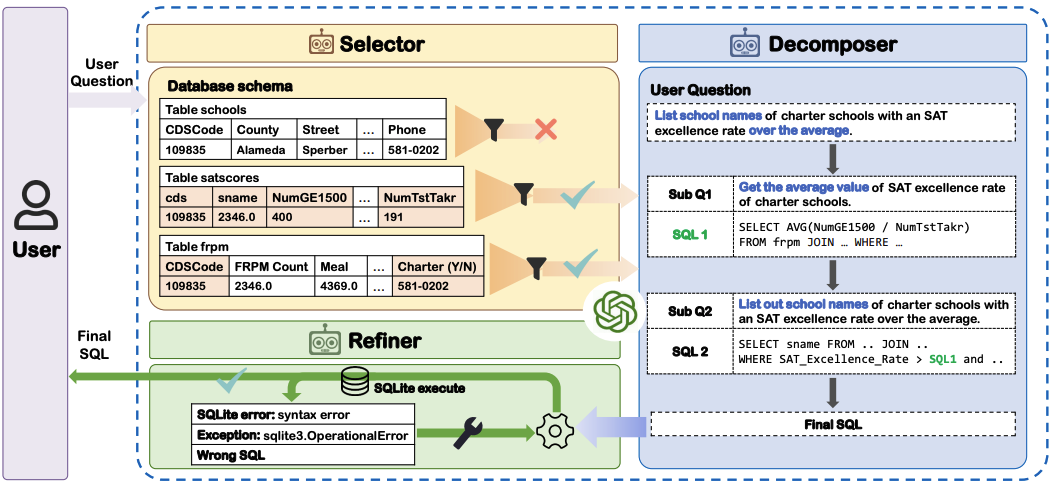
\includegraphics[scale=0.45]{images/wang2025_mac_sql.png}
  \end{center}
  \caption{\label{fig:wang2025_mac_sql}Visão geral do framework MAC-SQL. (Fonte: \citeonline{wang2025macsql})}
\end{figure}

A viabilidade dessa abordagem para modelos compactos é confirmada pelo desenvolvimento do \textit{SQL-Llama}. Ao realizar o \textit{fine-tuning} de um modelo de apenas 7B parâmetros com instruções específicas para o comportamento de agentes, o sistema atinge acurácia comparável à do GPT-4 em sua configuração padrão \cite{wang2025macsql}. Assim, a orquestração multiagente atua como um amplificador cognitivo, permitindo que SLMs superem limitações intrínsecas e alcancem o estado da arte \cite{wang2025macsql}.

% ---
% Capitulos de exemplo
% ---
\chapter{Lorem ipsum dolor sit amet}

% ---
\section{Aliquam vestibulum fringilla lorem}a
% ---

\lipsum[1]

\subsection{Aliquam vestibulum fringilla lorem}

\lipsum[2]

\subsubsection{Aliquam vestibulum fringilla lorem}

\lipsum[3]


\chapter{Lectus lobortis condimentum}

% ---
\section{Vestibulum ante ipsum primis in faucibus orci luctus et ultrices
  posuere cubilia Curae}
% ---

\lipsum[21-22]


\chapter{Nam sed tellus sit amet lectus urna ullamcorper tristique interdum
  elementum}

\section{Pellentesque sit amet pede ac sem eleifend consectetuer}

\lipsum[24]

% ---
% Finaliza a parte no bookmark do PDF, para que se inicie o bookmark na raiz
% ---
% \bookmarksetup{startatroot}% 
% ---

% ---
% Conclusão
% ---
\chapter{Conclusão}
% \addcontentsline{toc}{chapter}{Conclusão}

\lipsum[31-33]

% ----------------------------------------------------------
% ELEMENTOS PÓS-TEXTUAIS
% ----------------------------------------------------------
\postextual


% ----------------------------------------------------------
% Referências bibliográficas
% ----------------------------------------------------------
\bibliography{references}


% ----------------------------------------------------------
% Glossário
% ----------------------------------------------------------
%
% Consulte o manual da classe abntex2 para orientações sobre o glossário.
%
%\glossary

% ----------------------------------------------------------
% Apêndices
% ----------------------------------------------------------

% ---
% Apêndices (elemento opcional)
%
% São textos ou documentos elaborados pelo autor do trabalho a fim complementar
% a sua argumentação.
% ---
\begin{apendicesenv}

  % Imprime uma página indicando o início dos apêndices
  \partapendices

  % ----------------------------------------------------------
  \chapter{Quisque libero justo}
  % ----------------------------------------------------------

  \lipsum[50]

\end{apendicesenv}
% ---


% ----------------------------------------------------------
% Anexos (elemento opcional)
%
% São textos ou documentos, não elaborado pelo autor do trabalho que podem servir como
% ilustração, comprovação ou que contribua de forma relevante com o conteúdo já apresentado.
% ----------------------------------------------------------

% ---
% Inicia os anexos
% ---
\begin{anexosenv}

  % Imprime uma página indicando o início dos anexos
  \partanexos

  % ---
  \chapter{Morbi ultrices rutrum lorem.}
  % ---
  \lipsum[30]

\end{anexosenv}


% ----------------------------------------------------------
% Trabalhos publicados pelo autor
%
% Elemento obrigatório para as dissertações e teses do Programa
% de Pós-graduação em Ciência da Computação da UEL.
% (TCCs e monografias não precisam incluir essa seção)
% ----------------------------------------------------------
\chapter*{Trabalhos Publicados pelo Autor}
\addcontentsline{toc}{chapter}{Trabalhos Publicados pelo Autor}

\noindent
Trabalhos publicados pelo autor durante o programa.

% Elemento OBRIGATÓRIO somente para teses de doutorado e dissertações de mestrado no template DC/UEL).
% Listar publicações principais do trabalho (i.e., diretamente relacionados ao tema) e complementares, quando existirem.
% Listar em ordem decrescente de importância e/ou em ordem decrescente de ano de publicação.

\vspace{12pt}

\noindent
Publicações principais do trabalho.

\begin{enumerate}

  \item Jose da silva, autor2 da silva, orientador da silva, \textbf{Título do artigo}, local onde foi
        publicado, mês/ano, editora, número de página, isbn, etc. (Qualis CC 2017, xx)

  \item Jose da silva, autor2 da silva, orientador da silva, \textbf{Título do artigo}, local onde foi
        publicado, mês/ano, editora, número de página, isbn, etc. (Qualis CC 2017, xx)

  \item Jose da silva, autor2 da silva, orientador da silva, \textbf{Título do artigo}, local onde foi
        publicado, mês/ano, editora, número de página, isbn, etc. (Qualis CC 2017, xx)

\end{enumerate}

\noindent
Publicações complementares.

\begin{enumerate}

  \item Jose da silva, autor2 da silva, orientador da silva, \textbf{Título do artigo}, local onde foi
        publicado, mês/ano, editora, número de página, isbn, etc. (Qualis CC 2017, xx)

  \item Jose da silva, autor2 da silva, orientador da silva, etc. \textbf{Título do artigo}, local onde foi
        publicado, mês/ano, editora, número de página, isbn, (Qualis CC 2017, xx)

\end{enumerate}


%---------------------------------------------------------------------
% INDICE REMISSIVO (elemento opcional)
%---------------------------------------------------------------------
% Requer incluir instruções \index{...} no decorrer do texto, para marcar os termos a serem indexados

\printindex

\end{document}
